\documentclass{article}

\usepackage{titlesec}

\usepackage{amsmath}
\usepackage{amssymb}

\usepackage{booktabs}
\usepackage{float}
\usepackage{colortbl}
\usepackage{xcolor}

\usepackage{a4wide}
\usepackage{setspace}
\usepackage{geometry}
\usepackage{parskip}

\usepackage{multirow}
\usepackage{adjustbox}
\usepackage{graphicx}

\usepackage{hyperref}
\hypersetup{
    colorlinks=true,
    linkcolor=black,
    urlcolor=blue
}

\DeclareRobustCommand{\bbone}{\text{\usefont{U}{bbold}{m}{n}1}}

\DeclareMathOperator{\EX}{\mathbb{E}}

\titleformat*{\subsection}{\normalfont}

\author{Yu Xia \\ ID: yx5262}
\title{Yu Xia's Answer for Problem Set 5}
\date{Fall 2022}

\begin{document}
\maketitle

\nocite{*}

\section*{1}

\subsection*{(a)}

\fbox{%
\parbox[c]{\textwidth}{\
\begin{equation*}
    \begin{aligned}
    & \max_{\left(x_{0},x_{1}\right)}
      \sqrt{x_{0}}+\sqrt{x_{1}} \\
     \text{subject to}\\
    &   x_{0}=e_{0}=121,\\
    &   x_{1}=e_{1}=49,\\
    &   x_{0}\geqslant0, x_{1}\geqslant0.
    \end{aligned}
\end{equation*}%
}}

Plug in we have: 

$\boxed{V(121, 49)=\sqrt{121}+\sqrt{49}=11+7=18}$

\begin{figure}[H]
    \begin{center}
        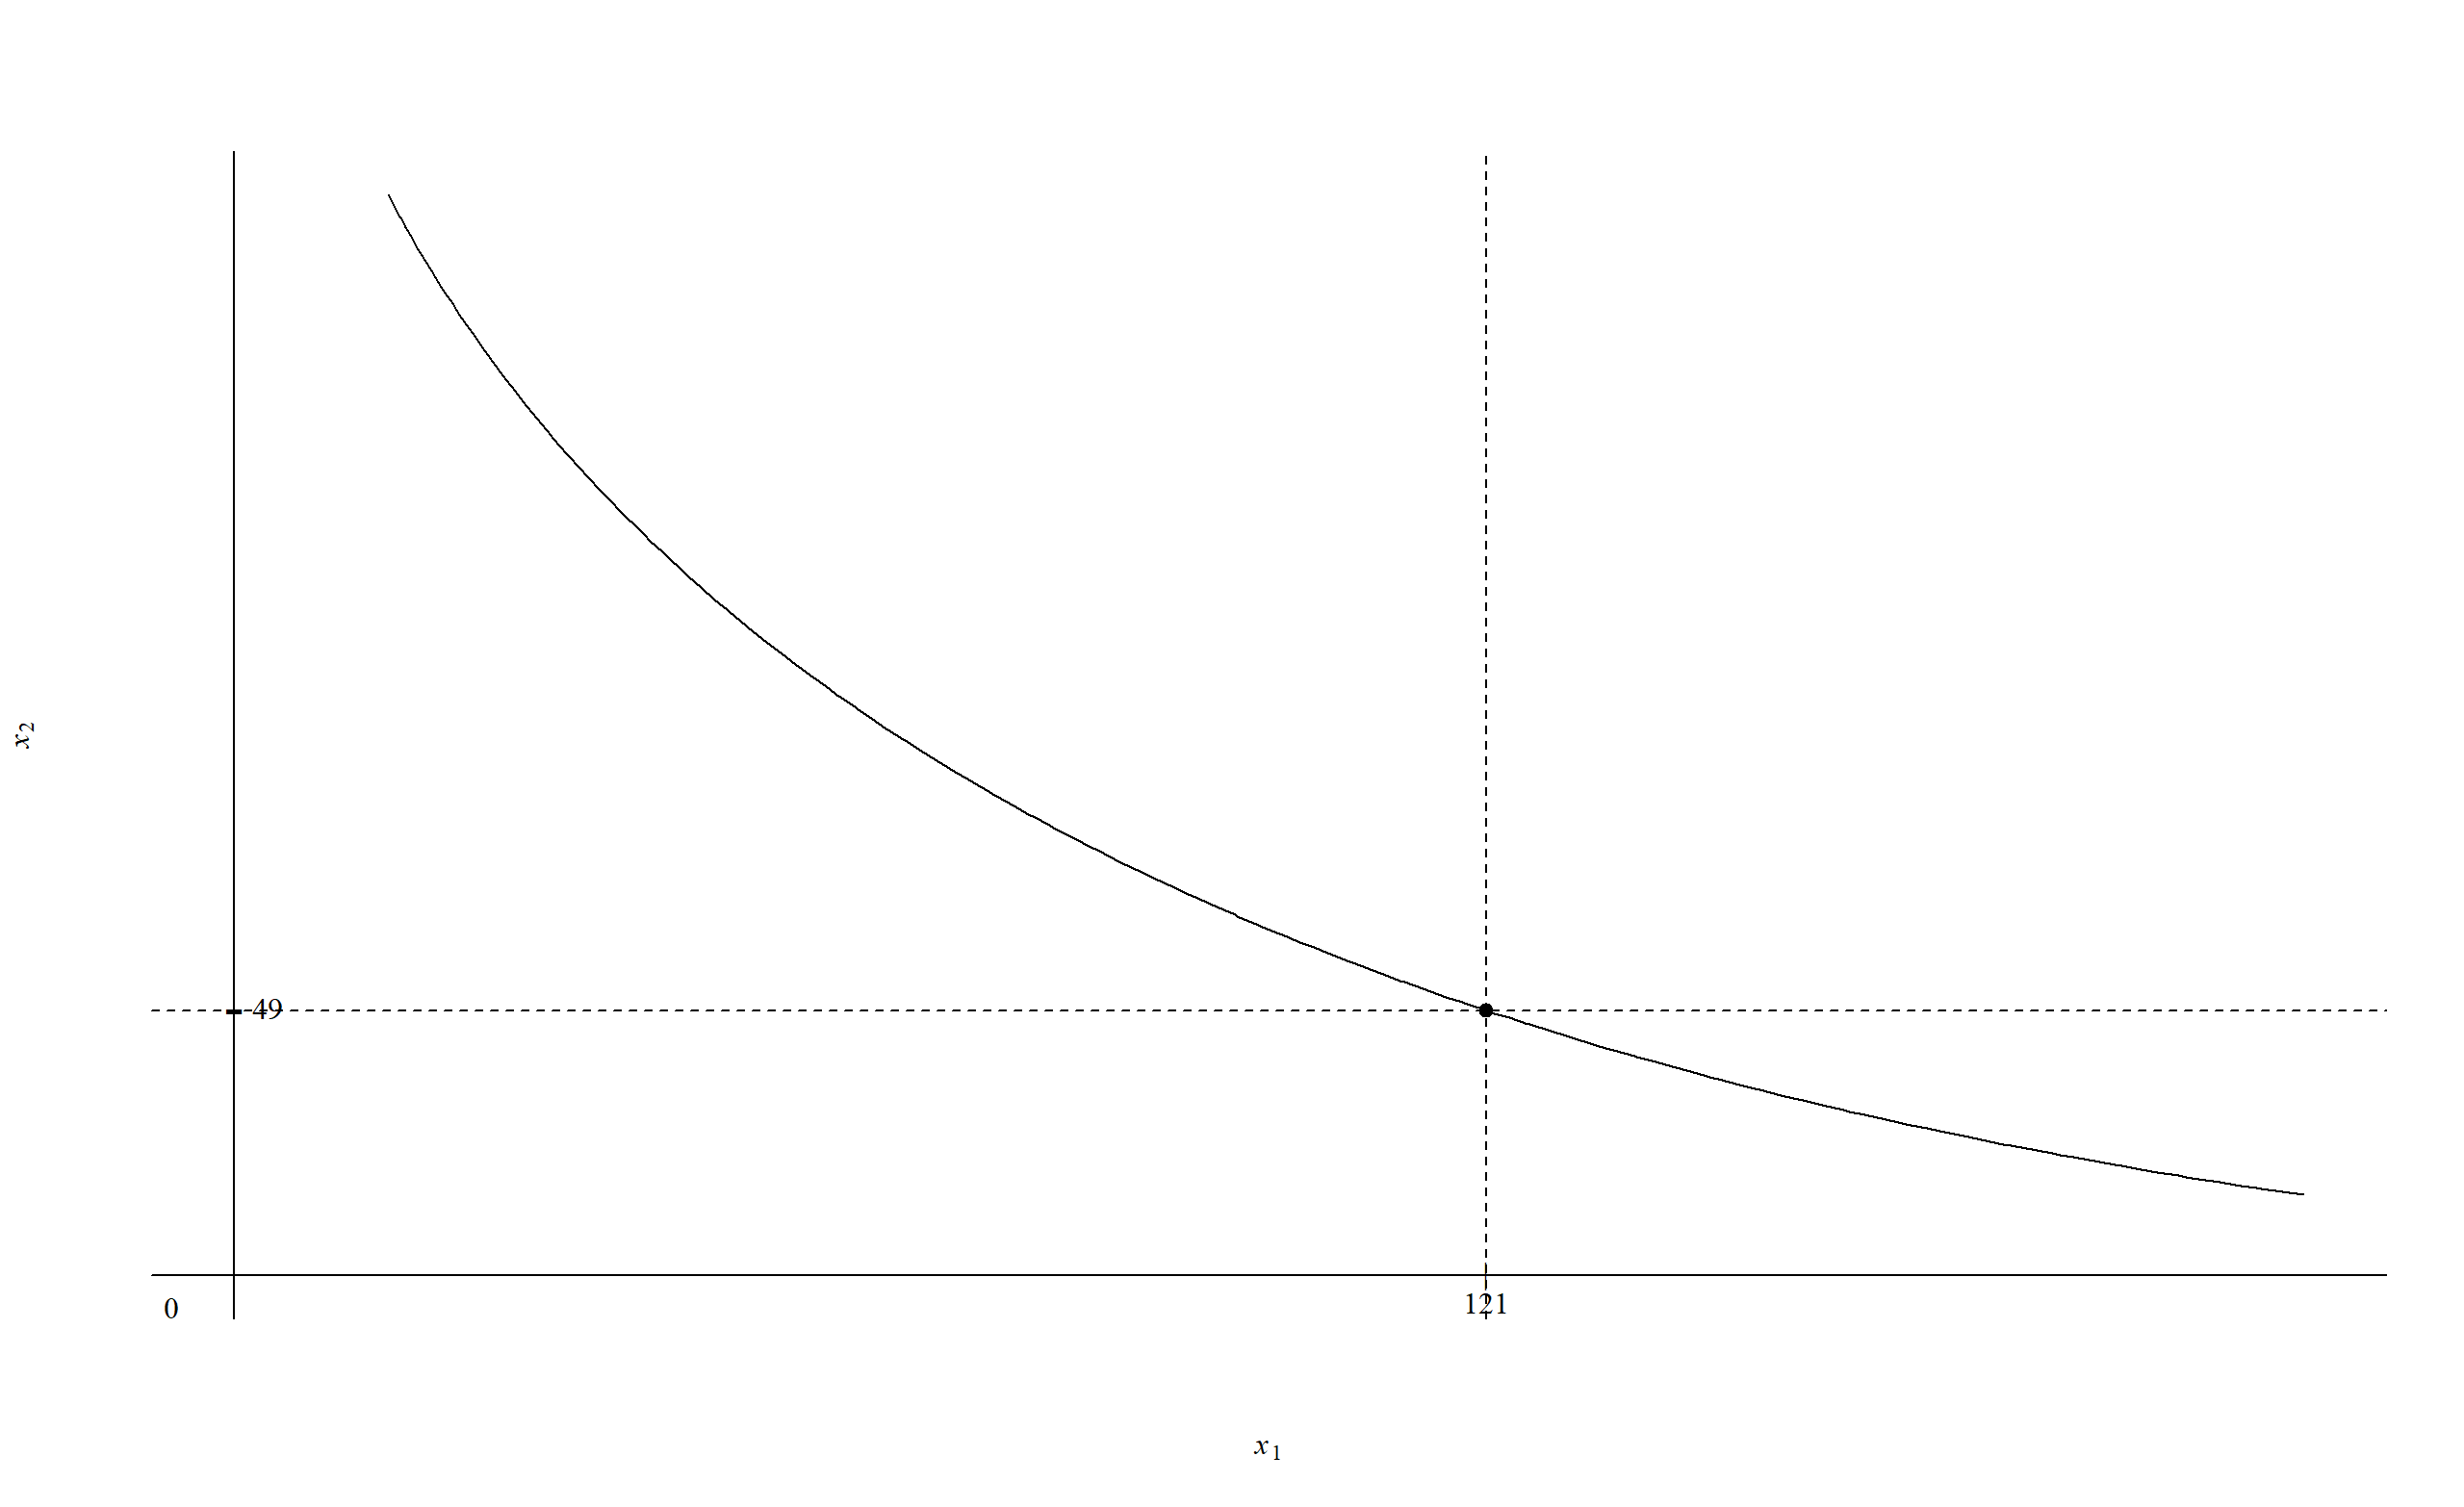
\includegraphics[width=.85\textwidth]{figures/figure1a.png}
    \end{center}
    \caption{Consumer's indifference curve through the optimal consumption bundle of 1(a)}
    \label{fig:graph}
\end{figure}

\subsection*{(b)}

The payoff matrix is:

$R=\begin{pmatrix}
    r_{11} & r_{12} \\
    r_{21} & r_{22}
\end{pmatrix}=\begin{pmatrix}
    1+r & 1 \\
    1+r & 1
\end{pmatrix}$

The asset prices are $(1,1)$.

The consumer's problem is:

\fbox{%
\parbox[c]{\textwidth}{\
\begin{equation*}
    \begin{aligned}
    & \max_{\left(x_{0},x_{1}\right)}
      \sqrt{x_{0}}+\sqrt{x_{1}} \\
     \text{subject to}\\
    &   x_{0}+b=121,\\
    &   x_{1}=49+\left(1+r\right)b,\\
    &   x_{0}\geqslant0, x_{1}\geqslant0.
    \end{aligned}
\end{equation*}%
}}

$b=121-x_{0}$

$x_{1}=49+\left(1+r\right)\left(121-x_{0}\right)=49+121\left(1+r\right)-x_{0}\left(1+r\right)$

$x_{0}\left(1+r\right)+x_{1}=49+121\left(1+r\right)$, the budget constraint.

$MU_{0}=\dfrac{1}{2}\left(x_{0}\right)^{-\dfrac{1}{2}}=\dfrac{1}{2}\cdot\dfrac{1}{\sqrt{x_{0}}}$

$MU_{1}=\dfrac{1}{2}\left(x_{1}\right)^{-\dfrac{1}{2}}=\dfrac{1}{2}\cdot\dfrac{1}{\sqrt{x_{1}}}$

MRS$=\dfrac{MU_{0}}{MU_{1}}=\dfrac{\dfrac{1}{2}\cdot\dfrac{1}{\sqrt{x_{0}}}}{\dfrac{1}{2}\cdot\dfrac{1}{\sqrt{x_{1}}}}=\dfrac{\dfrac{1}{\sqrt{x_{0}}}}{\dfrac{1}{\sqrt{x_{1}}}}=\dfrac{1}{\dfrac{\sqrt{x_{0}}}{\sqrt{x_{1}}}}=\dfrac{\sqrt{x_{1}}}{\sqrt{x_{0}}}=\sqrt{\dfrac{x_{1}}{x_{0}}}$

On the other hand,

MRS$=1+r$

$\therefore\sqrt{\dfrac{x_{1}}{x_{0}}}=1+r$

$\implies \dfrac{x_{1}}{x_{0}}=\left(1+r\right)^{2}$

$\implies x_{1}=\left(1+r\right)^{2}x_{0}$

Plug into constraint:

$x_{0}\left(1+r\right)+\left(1+r\right)^{2}x_{0}=49+121\left(1+r\right)$

$\implies x_{0}+x_{0}\left(1+r\right)=\dfrac{49}{1+r}+121$

$\implies x_{0}\left(2+r\right)=\dfrac{49}{1+r}+121$

$x_{0}=\dfrac{49}{\left(1+r\right)\left(2+r\right)}+\dfrac{121}{2+r}$

$x_{1}=\left(1+r\right)^{2}\left(\dfrac{49}{\left(1+r\right)\left(2+r\right)}+\dfrac{121}{2+r}\right)=\dfrac{49\left(1+r\right)}{2+r}+\dfrac{121\left(1+r\right)^{2}}{2+r}=\dfrac{49\left(1+r\right)+121\left(1+r\right)^{2}}{2+r}$

$\because r=0.03$

$\therefore$ The consumer's problem is:

\fbox{%
\parbox[c]{\textwidth}{\
\begin{equation*}
    \begin{aligned}
    & \max_{\left(x_{0},x_{1}\right)}
      \sqrt{x_{0}}+\sqrt{x_{1}} \\
     \text{subject to}\\
    &   x_{0}+b=121,\\
    &   x_{1}=49+1.03b,\\
    &   x_{0}\geqslant0, x_{1}\geqslant0.
    \end{aligned}
\end{equation*}%
}}

The budget constraint: $1.03x_{0}+x_{1}=49+121\times1.03=173.63$

$x_{0}=\dfrac{49}{1.03\times2.03}+\dfrac{121}{2.03}\approx\boxed{83.0408}$

$x_{1}=\dfrac{49\times1.03+121\left(1.03\right)^{2}}{2.03}\approx\boxed{88.09798}$

$b=121-x_{0}\approx\boxed{37.9592}$

The maximal utility level is:

\begin{equation*}
    \begin{split}
        V\left(x_{0},x_{1}\right) & = V\left(\dfrac{49}{\left(1+r\right)\left(2+r\right)}+\dfrac{121}{2+r}, \dfrac{49\left(1+r\right)+121\left(1+r\right)^{2}}{2+r}\right) \\
        & = \sqrt{\dfrac{49}{\left(1+r\right)\left(2+r\right)}+\dfrac{121}{2+r}}+\sqrt{\dfrac{49\left(1+r\right)+121\left(1+r\right)^{2}}{2+r}} \\
        & = \sqrt{\dfrac{49}{1.03\times2.03}+\dfrac{121}{2.03}}+\sqrt{\dfrac{49\times1.03+121\left(1.03\right)^{2}}{2.03}} \\
        & \approx \boxed{18.49872}
    \end{split}
\end{equation*}

Check the corner solution:

If $x_{0}=0$, $0+x_{1}=49+121\left(1+r\right)\implies x_{1}=49+121\times1.03=173.63$

$V\left(0, 173.63\right)=\sqrt{173.63}\approx13.17687<V\left(\dfrac{49}{1.03\times2.03}+\dfrac{121}{2.03}, \dfrac{49\times1.03+121\times1.03^{2}}{2.03}\right)$

If $x_{1}=0$, $\left(1+r\right)x_{0}+0=49+121\left(1+r\right)\implies x_{0}=\dfrac{49}{1+r}+121=\dfrac{49}{1.03}+121\approx168.5728$

$V\left(\dfrac{49}{1+r}+121,0\right)=\sqrt{\dfrac{49}{1+r}+121}=\sqrt{\dfrac{49}{1.03}+121}\approx12.98356$\\

$V\left(\dfrac{49}{1.03\times2.03}+\dfrac{121}{2.03}, \dfrac{49\times1.03+121\times1.03^{2}}{2.03}\right)$

\begin{figure}[H]
    \begin{center}
        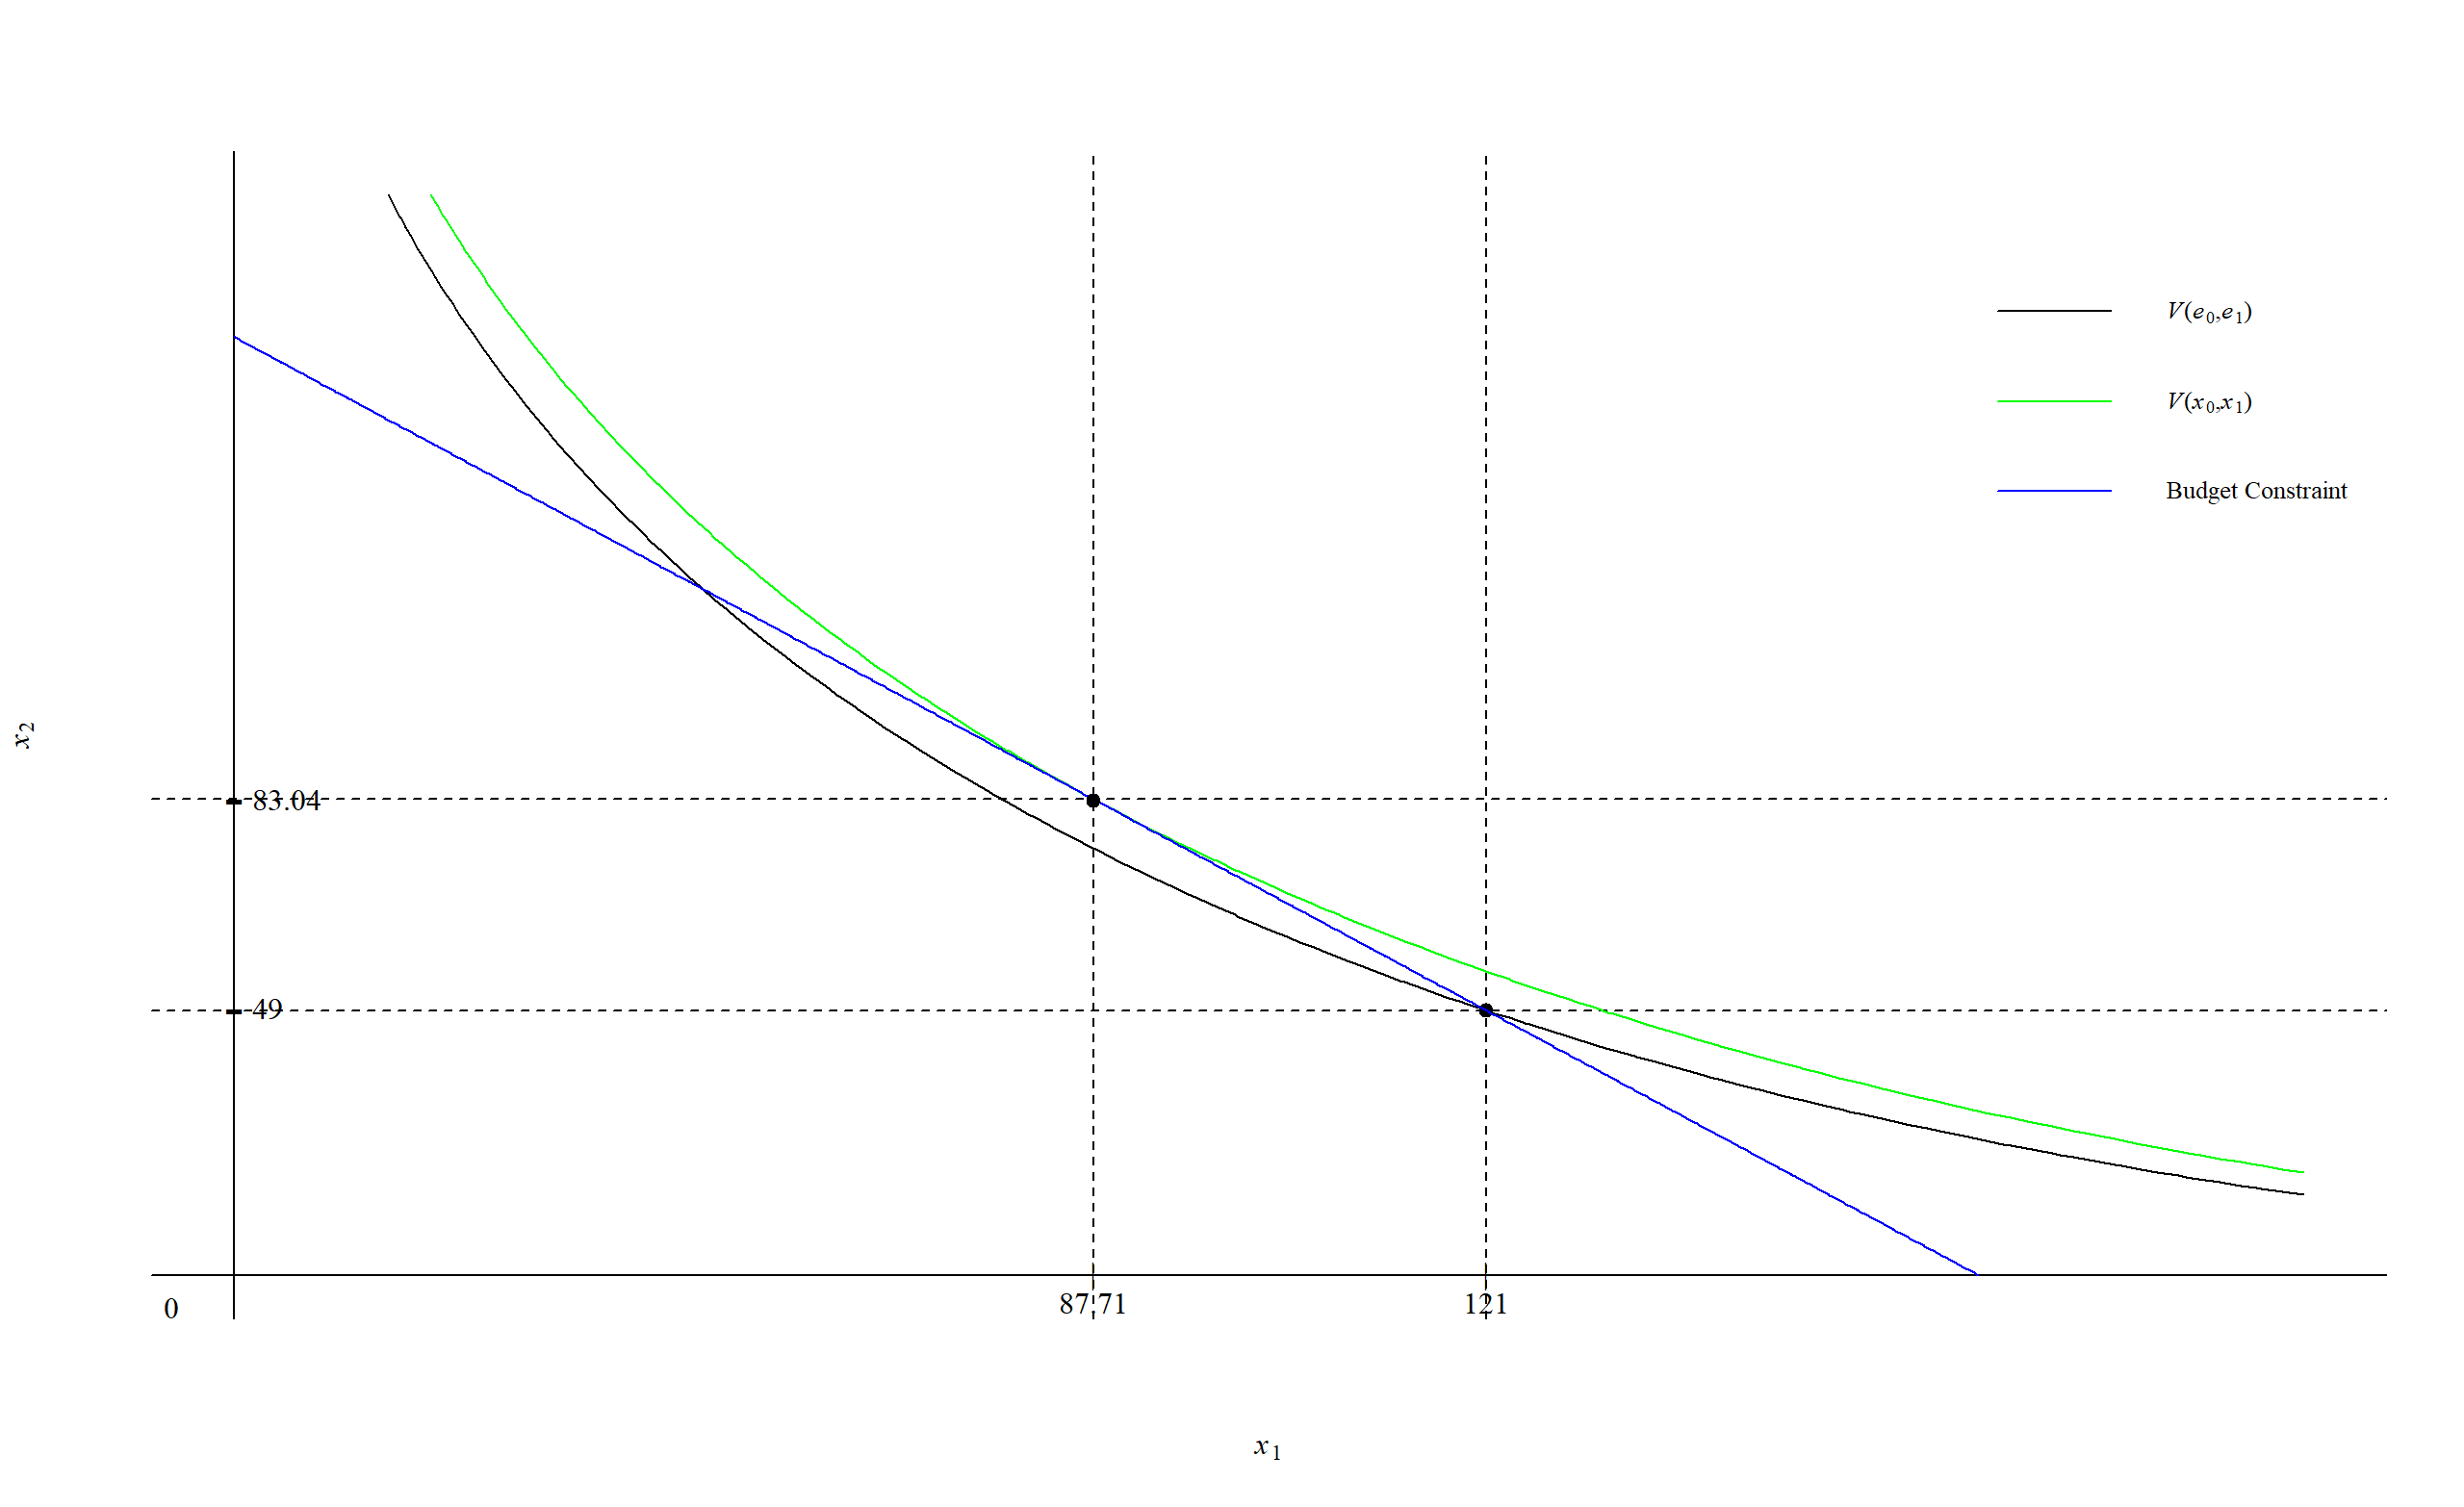
\includegraphics[width=.85\textwidth]{figures/figure1b.png}
    \end{center}
    \caption{Consumer's indifference curve through the optimal consumption bundle of 1(b)}
    \label{fig:graph}
\end{figure}

\subsection*{(c)}

The consumer is better off. We can see this from the diagram.

We can also prove it by math:

$V\left(121,49\right)=11+7=18<V\left(\dfrac{49}{\left(1+r\right)\left(2+r\right)}+\dfrac{121}{2+r}, \dfrac{49\left(1+r\right)+121\left(1+r\right)^{2}}{2+r}\right)$

The consumer saves part of his/her money, and invests in the risk-free bond at the same time, so that it pays back in the future. The consumer do so in order to maximize their utility.

\section*{2}

\subsection*{(a)}

\fbox{%
\parbox[c]{\textwidth}{\
\begin{equation*}
    \begin{aligned}
    & \max_{\left(x_{1},x_{2}\right)}
      \dfrac{1}{4}\sqrt{x_{1}}+\dfrac{3}{4}\sqrt{x_{2}} \\
     \text{subject to}\\
    &   x_{1}=e_{1}=121,\\
    &   x_{2}=e_{2}=49,\\
    &   x_{1}\geqslant0, x_{2}\geqslant0.
    \end{aligned}
\end{equation*}%
}}

Plug in we have:

$\boxed{V(121, 49)=\dfrac{1}{4}\sqrt{121}+\dfrac{3}{4}\sqrt{49}=\dfrac{1}{4}\times11+\dfrac{3}{4}\times7=\dfrac{11+21}{4}=\dfrac{32}{4}=\boxed{8}}$

\begin{figure}[H]
    \begin{center}
        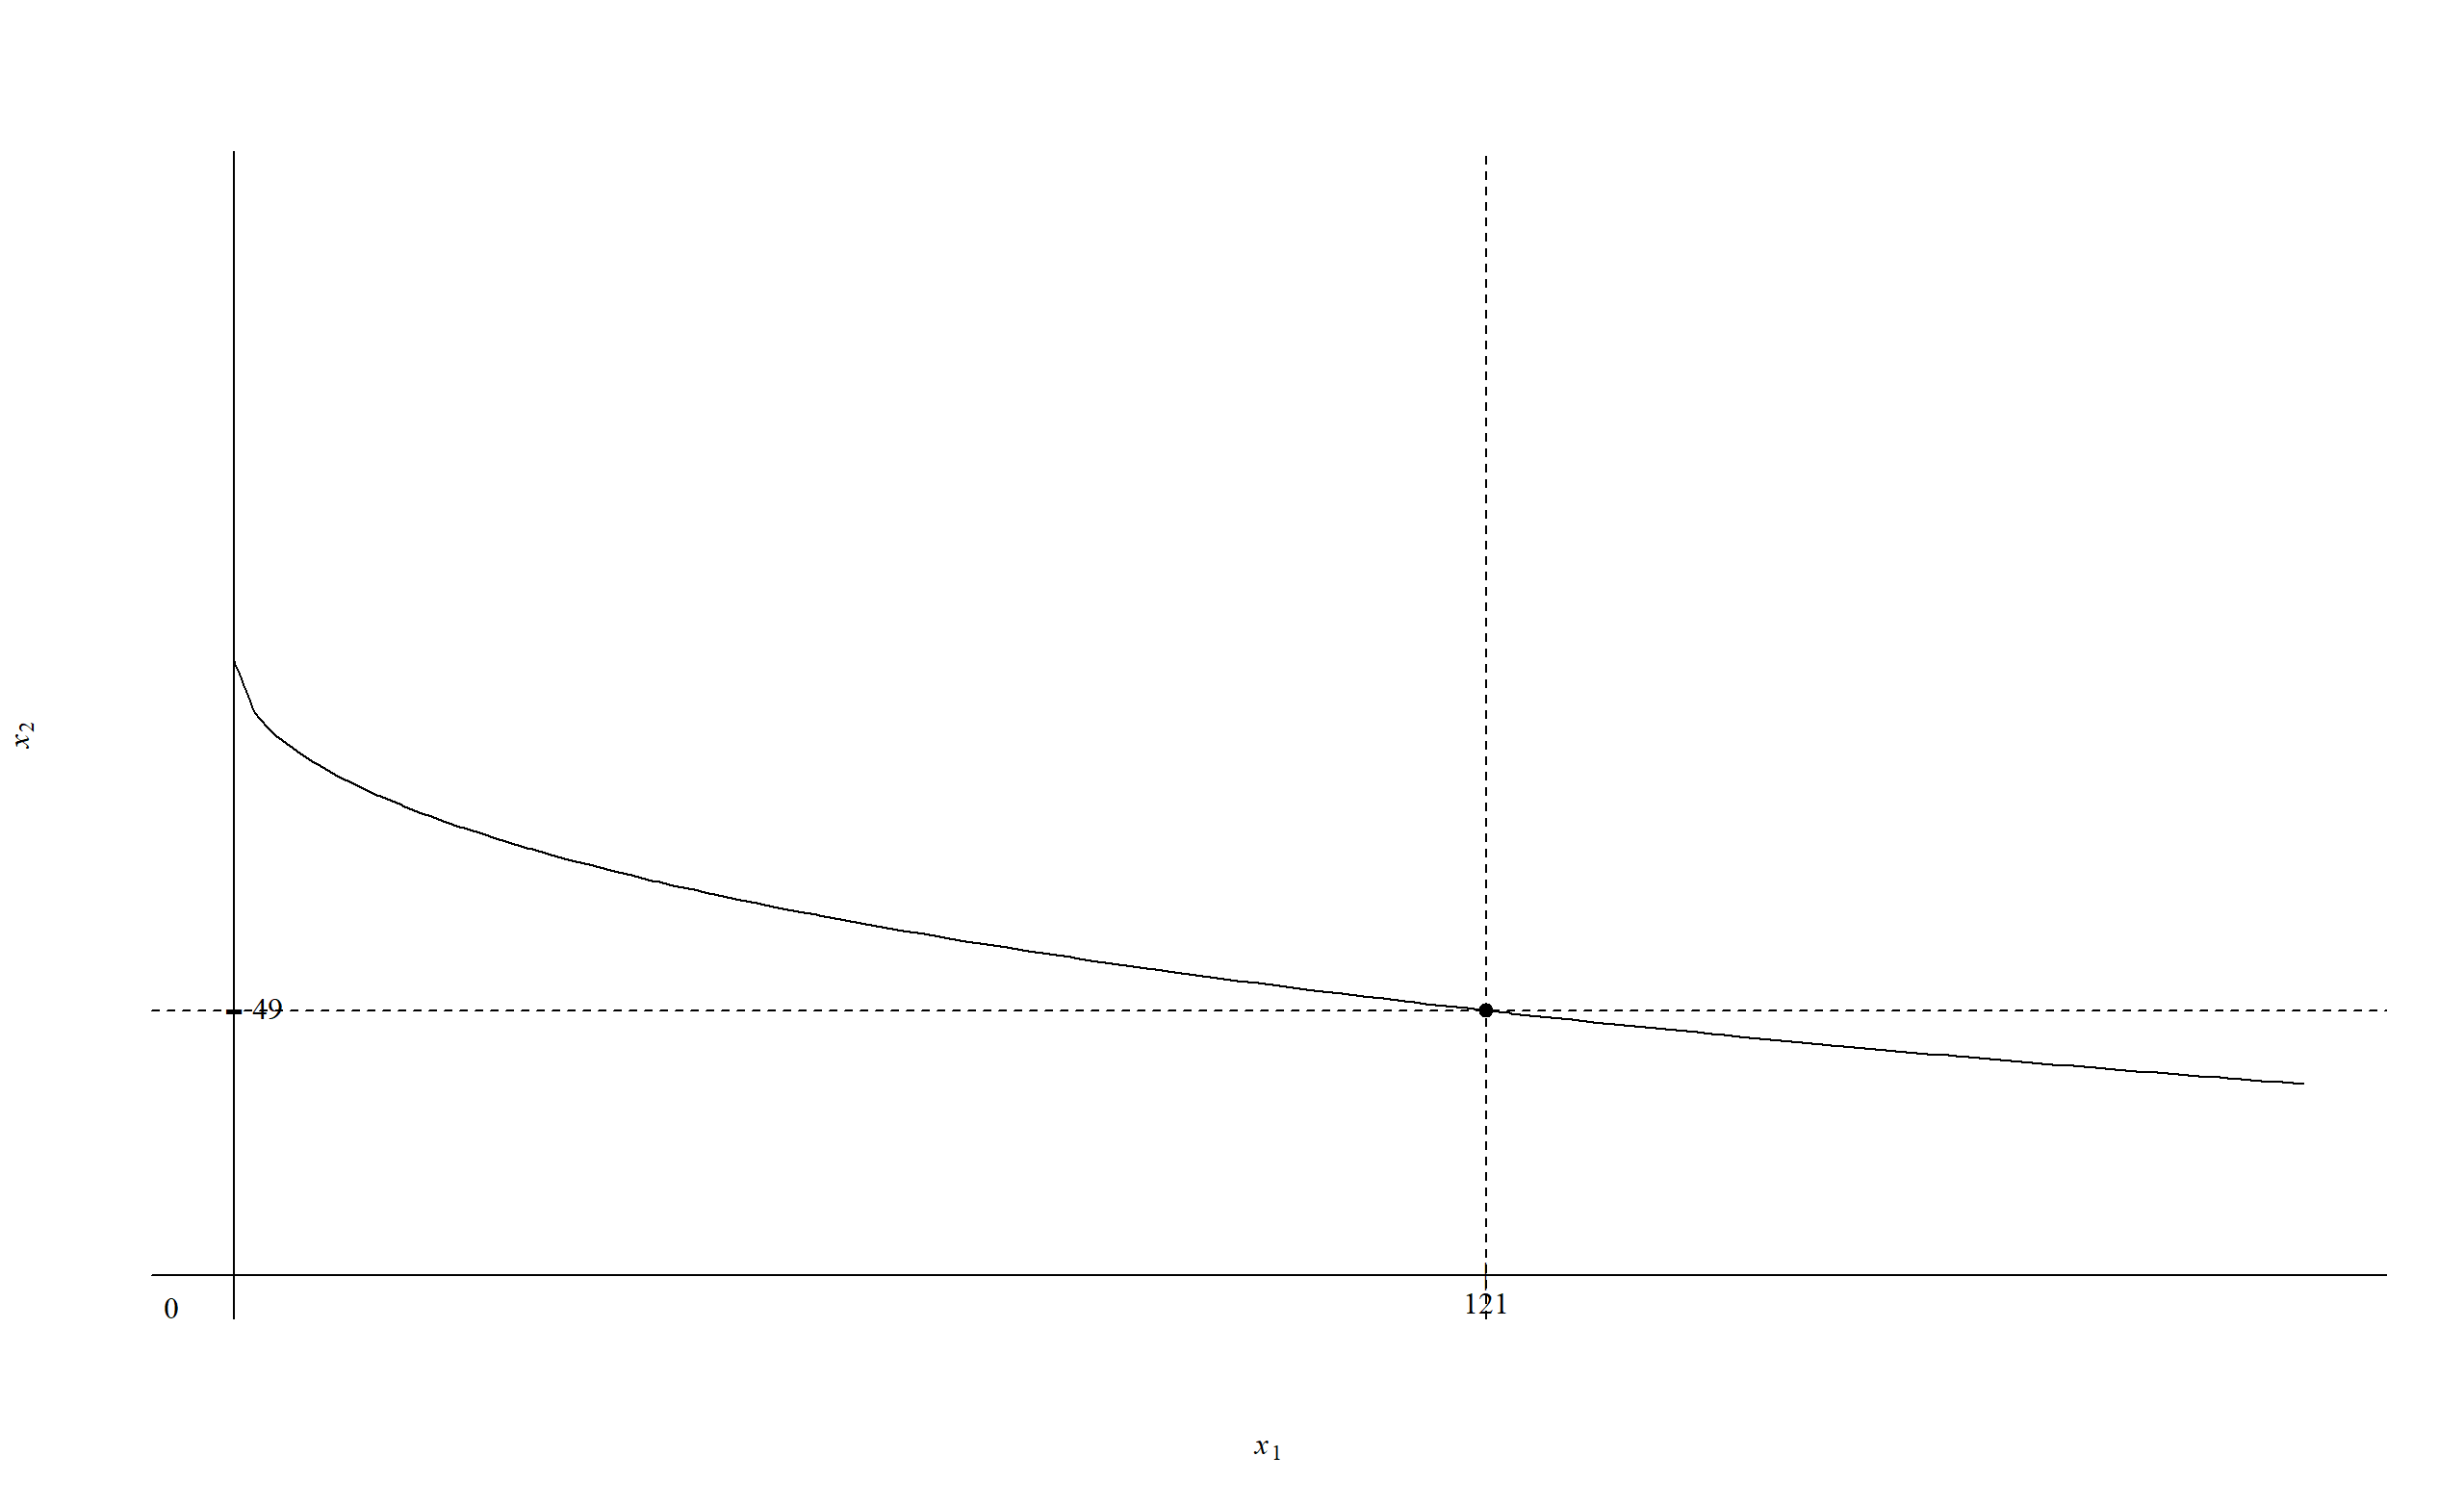
\includegraphics[width=.85\textwidth]{figures/figure2a.png}
    \end{center}
    \caption{consumer's indifference curve through the optimal consumption bundle of 2(a)}
    \label{fig:graph}
\end{figure}

\subsection*{(b)}

The payoff matrix is:

$R=\begin{pmatrix}
    r_{11} & r_{12} \\
    r_{21} & r_{22}
\end{pmatrix}=\begin{pmatrix}
    1+r & 1 \\
    1+r & 0
\end{pmatrix}$

The asset prices are $(1,q)$.

The consumer's problem is:

\fbox{%
\parbox[c]{\textwidth}{\
\begin{equation*}
    \begin{aligned}
    & \max_{\left(x_{1},x_{2}\right)}
      \dfrac{1}{4}\sqrt{x_{1}}+\dfrac{3}{4}\sqrt{x_{2}} \\
     \text{subject to}\\
    &   b+qk=0,\\
    &   x_{1}=121+\left(1+r\right)b+k,\\
    &   x_{2}=49+\left(1+r\right)b,\\
    &   x_{1}\geqslant0, x_{2}\geqslant0.
    \end{aligned}
\end{equation*}%
}}

$\implies b=-qk\implies x_{1}=121+\left(1+r\right)\left(-qk\right)+k=121-qk-rqk+k=121+\left(1-q-rq\right)k$

It also implies:

$x_{2}=49+\left(1+r\right)\left(-qk\right)=49-qk-rqk\implies x_{2}+qk+rqk=49\implies \left(1+r\right)qk=49-x_{2}$\\
$\implies k=\dfrac{49-x_{2}}{\left(1+r\right)q}$

Thus,

$\implies x_{1}=121+\left(1-q-rq\right)\cdot\dfrac{49-x_{2}}{\left(1+r\right)q}$

$\implies \left(1+r\right)qx_{1}=121\left(1+r\right)q+\left(1-q-rq\right)\left(49-x_{2}\right)$

$=121\left(1+r\right)q+\left(1-q-rq\right)\cdot49+\left(1-q-rq\right)\left(-x_{2}\right)$

$\implies \left(1+r\right)qx_{1}+\left(1-q-rq\right)x_{2}=121\left(1+r\right)q+49\left(1-q-rq\right)$

$\implies \left(1+r\right)qx_{1}+\left(1-q-rq\right)x_{2}=121q+121rq+49-49q-49rq$

$\implies \left(1+r\right)qx_{1}+\left(1-q-rq\right)x_{2}=72\left(1+r\right)q+49$, the budget constraint.

$MU_{1}=\dfrac{1}{4}\cdot\dfrac{1}{2}\left(x_{1}\right)^{-\dfrac{1}{2}}=\dfrac{1}{8}\cdot\dfrac{1}{\sqrt{x_{1}}}$

$MU_{2}=\dfrac{3}{4}\cdot\dfrac{1}{2}\left(x_{2}\right)^{-\dfrac{1}{2}}=\dfrac{3}{8}\cdot\dfrac{1}{\sqrt{x_{2}}}$

MRS$=\dfrac{MU_{1}}{MU_{2}}=\dfrac{\dfrac{1}{8}\cdot\dfrac{1}{\sqrt{x_{1}}}}{\dfrac{3}{8}\cdot\dfrac{1}{\sqrt{x_{2}}}}=\dfrac{\dfrac{1}{\sqrt{x_{1}}}}{\dfrac{3}{\sqrt{x_{2}}}}=\dfrac{1}{\dfrac{3\sqrt{x_{1}}}{\sqrt{x_{2}}}}=\dfrac{\sqrt{x_{2}}}{3\sqrt{x_{1}}}$

On the other hand,

MRS$=\dfrac{\left(1+r\right)q}{1-q-rq}$

$\therefore\dfrac{\sqrt{x_{2}}}{3\sqrt{x_{1}}}=\dfrac{\left(1+r\right)q}{1-q-rq}$

In order to generate a positive supply and demand for the risky asset, the expected value of the consumer's portfolio should be 0, that is,

$pk-qk=0$, where $p=0.25$ $\implies \boxed{q=\dfrac{1}{4}}$

Rewriting budget constraint:

$\dfrac{\left(1+r\right)x_{1}}{4}+\left(1-\dfrac{1}{4}-\dfrac{r}{4}\right)x_{2}=18\left(1+r\right)+49$

$\implies \left(1+r\right)x_{1}+\left(3-r\right)x_{2}=72\left(1+r\right)+196$

$\implies \left(1+r\right)x_{1}+\left(3-r\right)x_{2}=72+72r+196$

$\left(1+r\right)x_{1}+\left(3-r\right)x_{2}=268+72r$

Also,

$\dfrac{\sqrt{x_{2}}}{3\sqrt{x_{1}}}=\dfrac{\dfrac{1}{4}\left(1+r\right)}{1-\dfrac{1}{4}-\dfrac{1}{4}r}=\dfrac{1+r}{3-r}\implies\dfrac{x_{2}}{9x_{1}}=\dfrac{\left(1+r\right)^{2}}{\left(3-r\right)^{2}}\implies x_{2}=\dfrac{\left(1+r\right)^{2}}{\left(3-r\right)^{2}}\cdot9x_{1}$

The budget constraint becomes:

$\dfrac{1}{4}\left(1+r\right)x_{1}+\left(1-\dfrac{1}{4}-\dfrac{1}{4}r\right)\cdot\dfrac{\left(1+r\right)^{2}}{\left(3-r\right)^{2}}\cdot9x_{1}=72\left(1+r\right)\cdot\dfrac{1}{4}+49$

$\implies \dfrac{1}{4}\left(1+r\right)x_{1}+\dfrac{3-r}{4}\cdot\dfrac{\left(1+r\right)^{2}}{\left(3-r\right)^{2}}\cdot9x_{1}=72\left(1+r\right)\cdot\dfrac{1}{4}+\dfrac{4\times49}{4}$

$\implies \left(1+r\right)x_{1}+\dfrac{\left(1+r\right)^{2}}{3-r}\cdot9x_{1}=72\left(1+r\right)+4\times49$

$\implies \left(1+r\right)x_{1}\left(1+\dfrac{9\left(1+r\right)}{3-r}\right)=72\left(1+r\right)+196$

$\implies x_{1}\left(\dfrac{3-r}{3-r}+\dfrac{9+9r}{3-r}\right)=72+\dfrac{196}{1+r}$

$\implies x_{1}\cdot\dfrac{12+8r}{3-r}=72+\dfrac{196}{1+r}$

$\implies x_{1}\cdot\dfrac{3+2r}{3-r}=18+\dfrac{49}{1+r}=\dfrac{18+18r+49}{1+r}=\dfrac{67+18r}{1+r}$

$\implies x_{1}=\dfrac{67+18r}{1+r}\cdot\dfrac{3-r}{3+2r}$

$\implies x_{1}=\dfrac{\left(3-r\right)\left(67+18r\right)}{\left(1+r\right)\left(3+2r\right)}$

$x_{2}=\dfrac{\left(1+r\right)^{2}}{\left(3-r\right)^{2}}\cdot9x_{1}=\dfrac{\left(1+r\right)^{2}}{\left(3-r\right)^{2}}\cdot9\cdot\dfrac{\left(67+18r\right)\left(3-r\right)}{\left(1+r\right)\left(3+2r\right)}=\dfrac{1+r}{3-r}\cdot9\cdot\dfrac{67+18r}{3+2r}$

$x_{2}=\dfrac{9\left(1+r\right)\left(67+18r\right)}{\left(3-r\right)\left(3+2r\right)}$

$\left(1+r\right)b=x_{2}-49=\dfrac{9\left(1+r\right)\left(67+18r\right)}{\left(3-r\right)\left(3+2r\right)}-49$

$b=\dfrac{9\left(67+18r\right)}{\left(3-r\right)\left(3+2r\right)}-\dfrac{49}{1+r}$

$k=\dfrac{49-\dfrac{9\left(1+r\right)\left(67+18r\right)}{\left(3-r\right)\left(3+2r\right)}}{\left(1+r\right)\cdot\dfrac{1}{4}}=\dfrac{196}{1+r}-\dfrac{36\left(67+18r\right)}{\left(3-r\right)\left(3+2r\right)}$

The maximal utility level is:

\begin{equation*}
    \begin{split}
        V\left(x_{1},x_{2}\right) & = V\left(\dfrac{\left(3-r\right)\left(67+18r\right)}{\left(1+r\right)\left(3+2r\right)},\dfrac{9\left(1+r\right)\left(67+18r\right)}{\left(3-r\right)\left(3+2r\right)}\right) \\
        & = \dfrac{1}{4}\sqrt{\dfrac{\left(3-r\right)\left(67+18r\right)}{\left(1+r\right)\left(3+2r\right)}}+\dfrac{3}{4}\sqrt{\dfrac{9\left(1+r\right)\left(67+18r\right)}{\left(3-r\right)\left(3+2r\right)}} \\
        & = \dfrac{1}{4}\sqrt{\dfrac{\left(3-r\right)\left(67+18r\right)}{\left(1+r\right)\left(3+2r\right)}}+\dfrac{9}{4}\sqrt{\dfrac{\left(1+r\right)\left(67+18r\right)}{\left(3-r\right)\left(3+2r\right)}} \\
        & = \dfrac{1}{4}\sqrt{\dfrac{67+18r}{3+2r}}\left(\sqrt{\dfrac{3-r}{1+r}}+9\sqrt{\dfrac{1+r}{3-r}}\right)
    \end{split}
\end{equation*}

Check the corner solution:

If $x_{1}=0$, $0+\left(3-r\right)x_{2}=268+72r\implies x_{2}=\dfrac{268+72r}{3-r}$

$V\left(0, \dfrac{268+72r}{3-r}\right)=\dfrac{3}{4}\sqrt{\dfrac{268+72r}{3-r}}=\dfrac{3}{4}\sqrt{\dfrac{4\cdot\left(67+18r\right)}{3-r}}=\dfrac{3}{2}\sqrt{\dfrac{67+18r}{3-r}}$

If $x_{2}=0$, $\left(1+r\right)x_{1}+0=268+72r\implies x_{1}=\dfrac{268+72r}{1+r}$

$V\left(\dfrac{268+72r}{1+r},0\right)=\dfrac{1}{4}\sqrt{\dfrac{268+72r}{1+r}}=\dfrac{1}{2}\sqrt{\dfrac{67+18r}{1+r}}$

\begin{flalign*}
    \dfrac{V\left(\dfrac{\left(3-r\right)\left(67+18r\right)}{\left(1+r\right)\left(3+2r\right)},\dfrac{9\left(1+r\right)\left(67+18r\right)}{\left(3-r\right)\left(3+2r\right)}\right)}{V\left(0, \dfrac{268+72r}{3-r}\right)} & =\dfrac{\dfrac{1}{4}\sqrt{\dfrac{67+18r}{3+2r}}\left(\sqrt{\dfrac{3-r}{1+r}}+9\sqrt{\dfrac{1+r}{3-r}}\right)}{\dfrac{3}{2}\sqrt{\dfrac{67+18r}{3-r}}} &\\
    & =\dfrac{1}{4}\sqrt{\dfrac{67+18r}{3+2r}}\left(\sqrt{\dfrac{3-r}{1+r}}+9\sqrt{\dfrac{1+r}{3-r}}\right)\cdot\dfrac{2}{3}\sqrt{\dfrac{3-r}{67+18r}} &\\
    & =\dfrac{1}{4}\cdot\dfrac{2}{3}\sqrt{\dfrac{3-r}{3+2r}}\left(\sqrt{\dfrac{3-r}{1+r}}+9\sqrt{\dfrac{1+r}{3-r}}\right) &\\
    & =\dfrac{1}{6}\left(\dfrac{3-r}{\sqrt{\left(3+2r\right)\left(1+r\right)}}+9\sqrt{\dfrac{1+r}{3+2r}}\right)>1
\end{flalign*}

In the interval $r\in(0, 1]$, the fraction above minimizes at $r=1$ with value about $1.054093$.

\begin{flalign*}
    \dfrac{V\left(\dfrac{\left(3-r\right)\left(67+18r\right)}{\left(1+r\right)\left(3+2r\right)},\dfrac{9\left(1+r\right)\left(67+18r\right)}{\left(3-r\right)\left(3+2r\right)}\right)}{V\left(\dfrac{268+72r}{1+r},0\right)} & =\dfrac{\dfrac{1}{4}\sqrt{\dfrac{67+18r}{3+2r}}\left(\sqrt{\dfrac{3-r}{1+r}}+9\sqrt{\dfrac{1+r}{3-r}}\right)}{\dfrac{1}{2}\sqrt{\dfrac{67+18r}{1+r}}} &\\
    & =\dfrac{1}{4}\sqrt{\dfrac{67+18r}{3+2r}}\left(\sqrt{\dfrac{3-r}{1+r}}+9\sqrt{\dfrac{1+r}{3-r}}\right)\cdot2\sqrt{\dfrac{1+r}{67+18r}} &\\
    & =\dfrac{1}{2}\sqrt{\dfrac{1+r}{3+2r}}\left(\sqrt{\dfrac{3-r}{1+r}}+9\sqrt{\dfrac{1+r}{3-r}}\right) &\\
    & =\dfrac{1}{2}\left(\sqrt{\dfrac{3-r}{3+2r}}+9\dfrac{1+r}{\sqrt{\left(3+2r\right)\left(3-r\right)}}\right)\geqslant2
\end{flalign*}

In the interval $r\in(0, 1)$, the fraction above minimizes at about $r=0$ with value approximately $2$.

Hence, 

\begin{spacing}{1.7}
    \fbox{%
    \parbox[c]{.5\textwidth}{\
    $\begin{cases}
        x_{1}=\dfrac{\left(3-r\right)\left(67+18r\right)}{\left(1+r\right)\left(3+2r\right)}\\
        x_{2}=\dfrac{9\left(1+r\right)\left(67+18r\right)}{\left(3-r\right)\left(3+2r\right)}\\
        b=\dfrac{9\left(67+18r\right)}{\left(3-r\right)\left(3+2r\right)}-\dfrac{49}{1+r}\\
        k=\dfrac{196}{1+r}-\dfrac{36\left(67+18r\right)}{\left(3-r\right)\left(3+2r\right)}\\
        \max V=\dfrac{1}{4}\sqrt{\dfrac{67+18r}{3+2r}}\left(\sqrt{\dfrac{3-r}{1+r}}+9\sqrt{\dfrac{1+r}{3-r}}\right)
    \end{cases}$}%
    }
\end{spacing}

If $r=0.03$,

$x_{1}=\dfrac{67+18\times0.03}{1.03}\cdot\dfrac{3-0.03}{3+2\times0.03}\approx63.6442$

$x_{2}=\dfrac{9\times1.03\left(67+18\times0.03\right)}{\left(3-0.03\right)\left(3+2\times0.03\right)}\approx68.89107$

$b=\dfrac{9\left(67+18\times0.03\right)}{\left(3-0.03\right)\left(3+2\times0.03\right)}-\dfrac{49}{1.03}\approx19.31172$

$k=\dfrac{196}{1.03}-\dfrac{36\left(67+18\times1.03\right)}{\left(3-0.03\right)\left(3+2\times0.03\right)}\approx-77.24686$

$V\left(x_{1},x_{2}\right)=\dfrac{1}{4}\sqrt{\dfrac{67+18\times0.03}{3+2\times0.03}}\left(\sqrt{\dfrac{3-0.03}{1.03}}+9\sqrt{\dfrac{1.03}{3-0.03}}\right)\approx8.219481$

\subsection*{(c)}

\begin{figure}[H]
    \begin{center}
        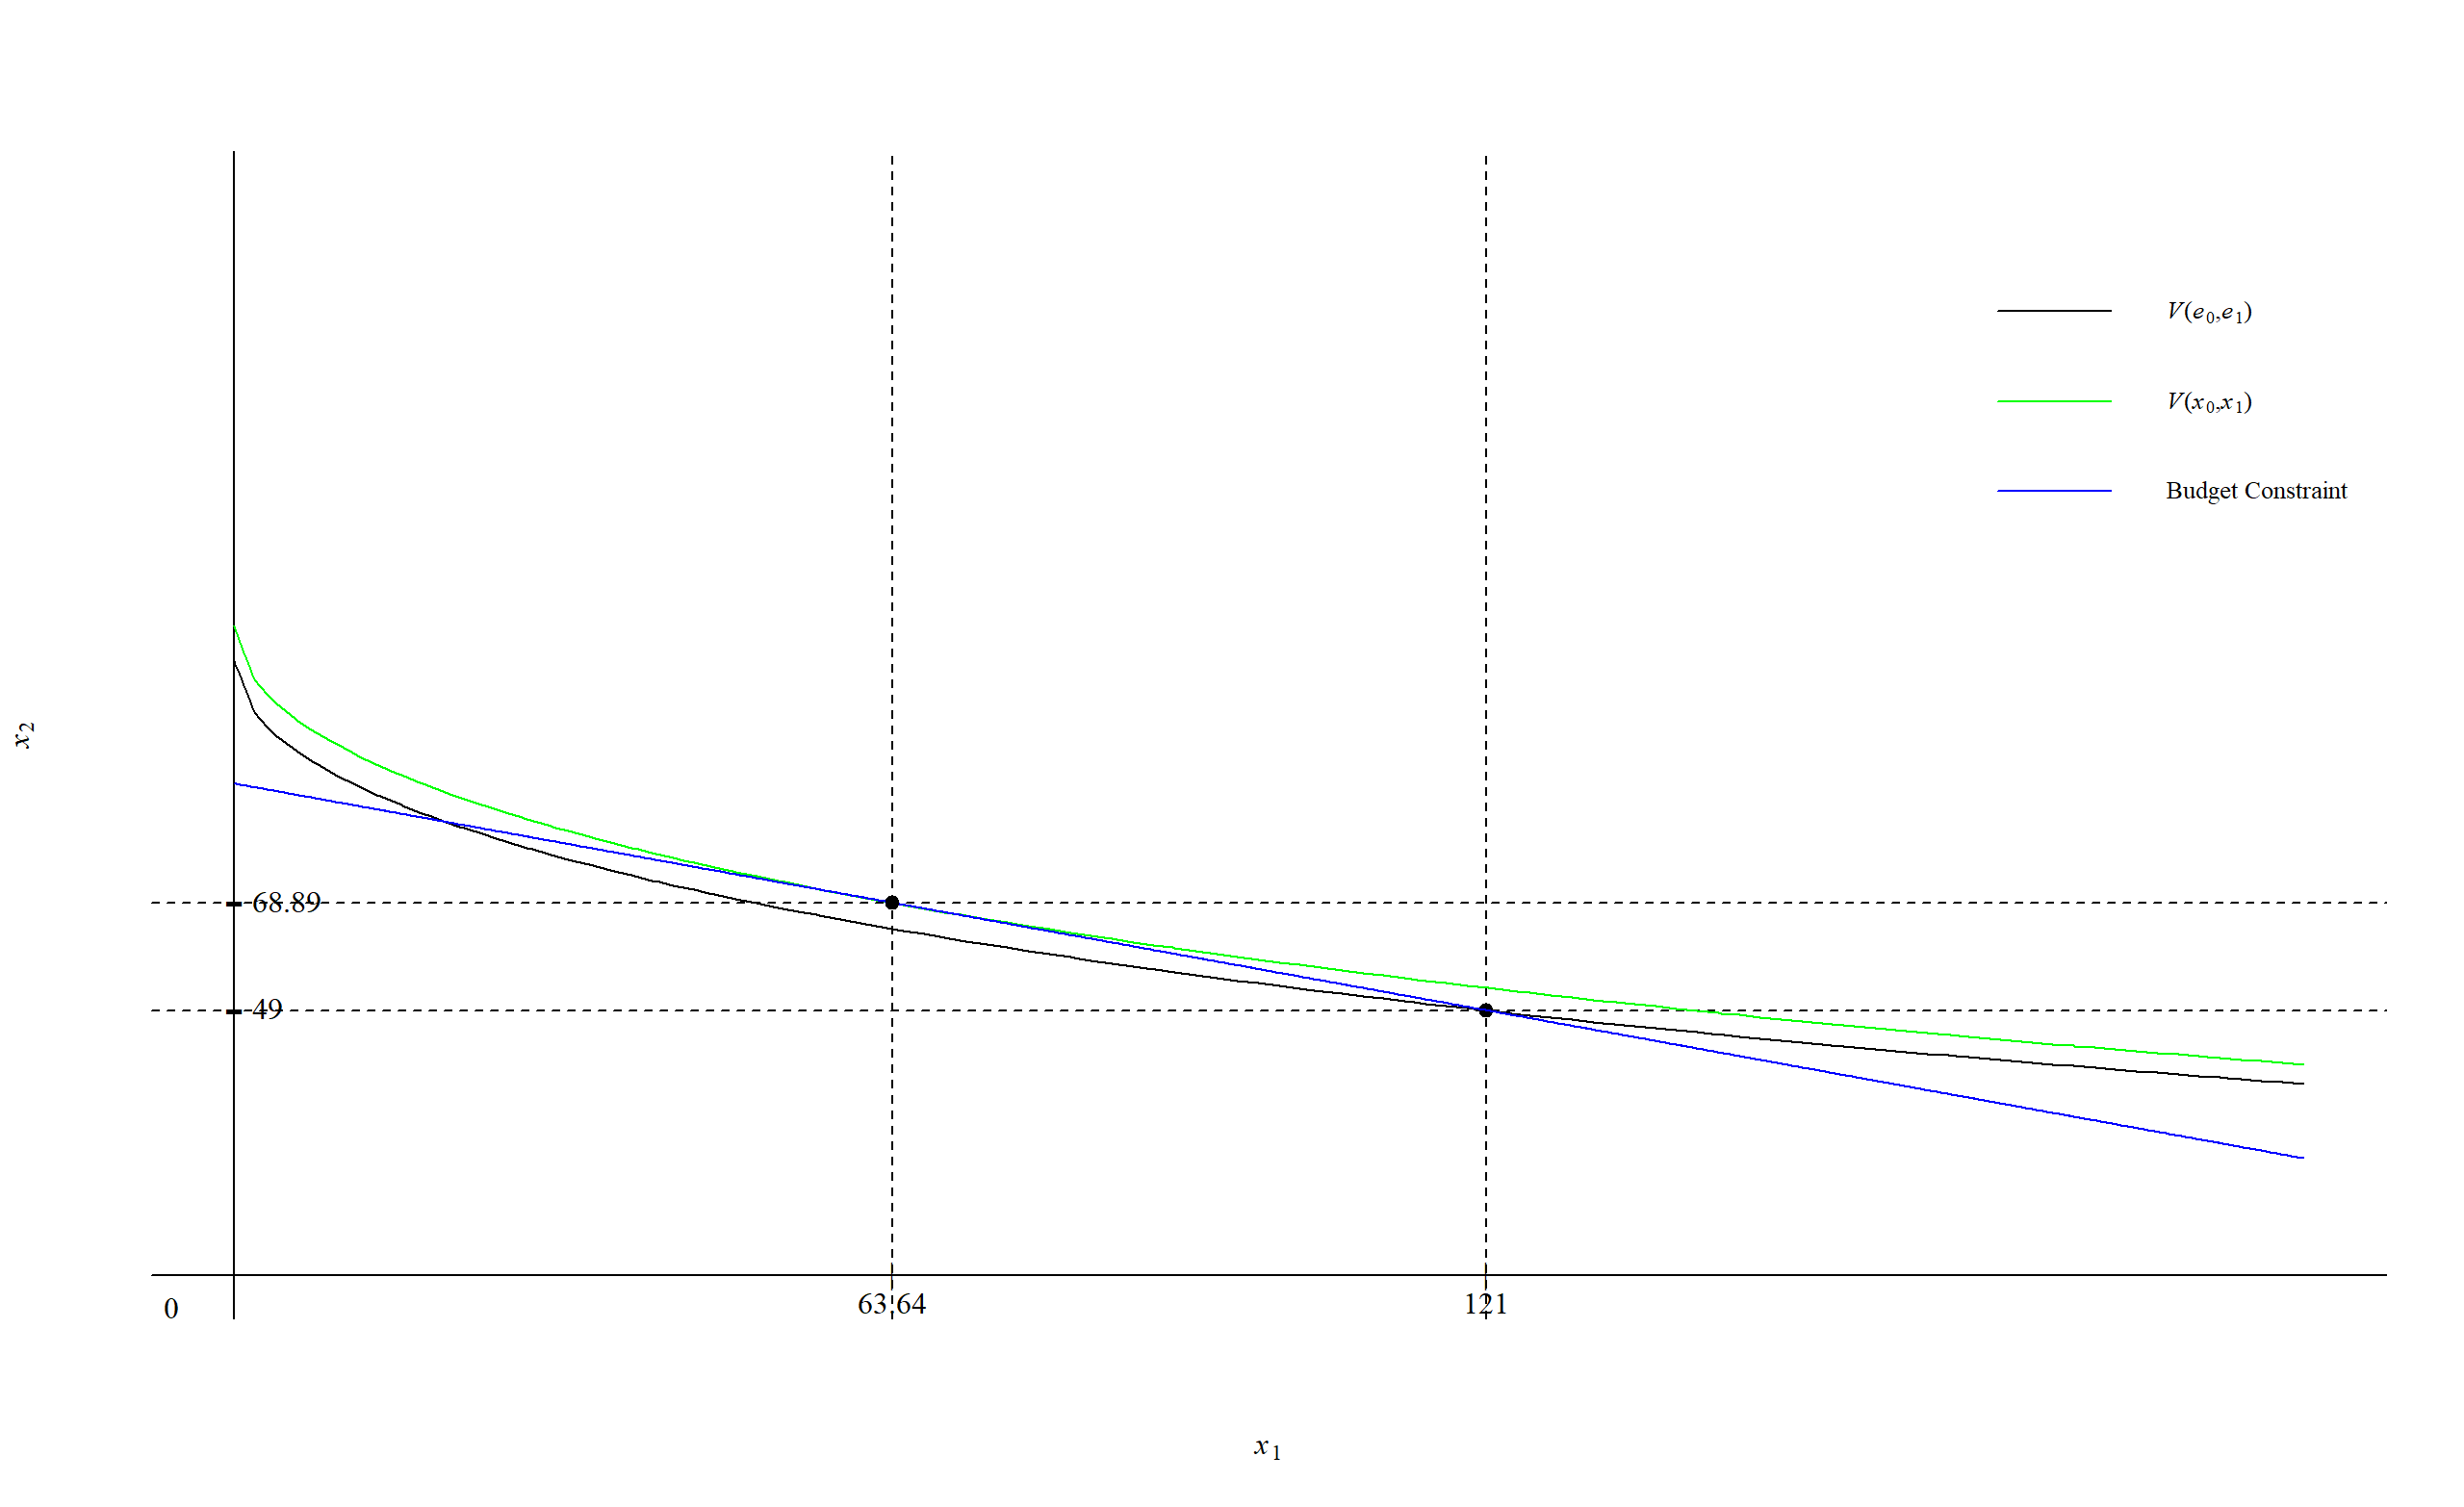
\includegraphics[width=.85\textwidth]{figures/figure2b.png}
    \end{center}
    \caption{consumer's indifference curve through the optimal consumption bundle of 2(b)}
    \label{fig:graph}
\end{figure}

\subsection*{(d)}

The consumer is better off. His/her indifference curve is higher, as shown in the figure above. We can also prove it by math that

$\dfrac{1}{4}\times11+\dfrac{3}{4}\times7=\dfrac{11}{4}+\dfrac{21}{4}=\dfrac{32}{4}=8$

While $\max V=\dfrac{1}{4}\sqrt{\dfrac{67+18r}{3+2r}}\left(\sqrt{\dfrac{3-r}{1+r}}+9\sqrt{\dfrac{1+r}{3-r}}\right)>8$.

$b=\dfrac{9\left(67+18r\right)}{\left(3-r\right)\left(3+2r\right)}-\dfrac{49}{1+r}>0$, which means the consumer has long position of bond, and short position on risky asset, in order to maximize his/her expected utility.

Also, $x_{1}=x_{2}$ doesn't hold generally. It implies that the consumer doesn't hedge all his/her risk.

\section*{3}

\subsection*{(a)}

\fbox{%
\parbox[c]{\textwidth}{\
\begin{equation*}
    \begin{aligned}
    & \max_{\left(x^{A}_{1},x^{A}_{2}\right)}
      \dfrac{1}{2}\ln{x^{A}_{1}}+\dfrac{1}{2}\ln{x^{A}_{2}} \\
     \text{subject to}\\
    &   \hat{p}_{1}x^{A}_{1}+\hat{p}_{2}x^{A}_{2}=\hat{p}_{1}+2\hat{p}_{2}.
    \end{aligned}
\end{equation*}%
}}

For Alice:

$MU^{A}_{1}=\dfrac{1}{2}\cdot\dfrac{1}{x^{A}_{1}}$

$MU^{A}_{2}=\dfrac{1}{2}\cdot\dfrac{1}{x^{A}_{2}}$

MRS$^{A}=\dfrac{MU^{A}_{1}}{MU^{A}_{2}}=MU^{A}_{1}\cdot\dfrac{1}{MU^{A}_{2}}=\dfrac{1}{2}\cdot\dfrac{1}{x^{A}_{1}}\cdot2x^{A}_{2}=\dfrac{x^{A}_{2}}{x^{A}_{1}}$

On the other hand, 

MRS$^{A}=\dfrac{\hat{p}_{1}}{\hat{p}_{2}}$

$\therefore \dfrac{x^{A}_{2}}{x^{A}_{1}}=\dfrac{\hat{p}_{1}}{\hat{p}_{2}}$

Substituting $x^{A}_{2}=\dfrac{\hat{p}_{1}}{\hat{p}_{2}}x^{A}_{1}$ into budget constraint for Alice:

$\hat{p}_{1}x^{A}_{1}+\hat{p}_{2}\dfrac{\hat{p}_{1}}{\hat{p}_{2}}x^{A}_{1}=\hat{p}_{1}+2\hat{p}_{2}$

$\implies \hat{p}_{1}x^{A}_{1}+\hat{p}_{1}x^{A}_{1}=\hat{p}_{1}+2\hat{p}_{2}$

$\implies 2\hat{p}_{1}x^{A}_{1}=\hat{p}_{1}+2\hat{p}_{2}$

$\implies x^{A}_{1}=\dfrac{\hat{p}_{1}+2\hat{p}_{2}}{2\hat{p}_{1}}=\boxed{\dfrac{1}{2}+\dfrac{\hat{p}_{2}}{\hat{p}_{1}}}$

$x^{A}_{2}=\dfrac{\hat{p}_{1}}{\hat{p}_{2}}x^{A}_{1}=\dfrac{\hat{p}_{1}}{\hat{p}_{2}}\left(\dfrac{1}{2}+\dfrac{\hat{p}_{2}}{\hat{p}_{1}}\right)=\boxed{\dfrac{\hat{p}_{1}}{2\hat{p}_{2}}+1}$

\subsection*{(b)}

\fbox{%
\parbox[c]{\textwidth}{\
\begin{equation*}
    \begin{aligned}
    & \max_{\left(x^{B}_{1},x^{B}_{2}\right)}
      \dfrac{1}{2}\ln{x^{B}_{1}}+\dfrac{1}{2}\ln{x^{B}_{2}} \\
     \text{subject to}\\
    &   \hat{p}_{1}x^{B}_{1}+\hat{p}_{2}x^{B}_{2}=3\hat{p}_{1}+\hat{p}_{2}.
    \end{aligned}
\end{equation*}%
}}

For Bob:

$MU^{B}_{1}=\dfrac{1}{2}\cdot\dfrac{1}{x^{B}_{1}}$

$MU^{B}_{2}=\dfrac{1}{2}\cdot\dfrac{1}{x^{B}_{2}}$

MRS$^{B}=\dfrac{MU^{B}_{1}}{MU^{B}_{2}}=MU^{B}_{1}\cdot\dfrac{1}{MU^{B}_{2}}=\dfrac{1}{2}\cdot\dfrac{1}{x^{B}_{1}}\cdot2x^{B}_{2}=\dfrac{x^{B}_{2}}{x^{B}_{1}}$

On the other hand, 

MRS$^{B}=\dfrac{\hat{p}_{1}}{\hat{p}_{2}}$

$\therefore \dfrac{x^{B}_{2}}{x^{B}_{1}}=\dfrac{\hat{p}_{1}}{\hat{p}_{2}}$

Substituting $x^{B}_{2}=\dfrac{\hat{p}_{1}}{\hat{p}_{2}}x^{B}_{1}$ into budget constraint for Bob:

$\hat{p}_{1}x^{B}_{1}+\hat{p}_{2}\dfrac{\hat{p}_{1}}{\hat{p}_{2}}x^{B}_{1}=3\hat{p}_{1}+\hat{p}_{2}$

$\implies \hat{p}_{1}x^{B}_{1}+\hat{p}_{1}x^{B}_{1}=3\hat{p}_{1}+\hat{p}_{2}$

$\implies 2\hat{p}_{1}x^{B}_{1}=3\hat{p}_{1}+\hat{p}_{2}$

$\implies x^{B}_{1}=\dfrac{3\hat{p}_{1}+\hat{p}_{2}}{2\hat{p}_{1}}=\boxed{\dfrac{3}{2}+\dfrac{\hat{p}_{2}}{2\hat{p}_{1}}}$

$x^{B}_{2}=\dfrac{\hat{p}_{1}}{\hat{p}_{2}}\left(\dfrac{3}{2}+\dfrac{\hat{p}_{2}}{2\hat{p}_{1}}\right)=\boxed{\dfrac{3\hat{p}_{1}}{2\hat{p}_{2}}+\dfrac{1}{2}}$

\subsection*{(c)}

The market for consumption in state 1: 

$x^{A}_{1}+x^{B}_{1}=e^{A}_{1}+e^{B}_{1}=1+3=4$

$\iff \dfrac{1}{2}+\dfrac{\hat{p}_{2}}{\hat{p}_{1}}+\dfrac{3}{2}+\dfrac{\hat{p}_{2}}{2\hat{p}_{1}}=4$

$\iff 2+\dfrac{2\hat{p}_{2}}{2\hat{p}_{1}}+\dfrac{\hat{p}_{2}}{2\hat{p}_{1}}=4$

$\iff \dfrac{3\hat{p}_{2}}{2\hat{p}_{1}}=2$

$\iff \dfrac{\hat{p}_{2}}{\hat{p}_{1}}=2\times\dfrac{2}{3}$

$\iff \boxed{\dfrac{\hat{p}_{1}}{\hat{p}_{2}}=\dfrac{3}{4}}$

$x^{A}_{1}=\dfrac{1}{2}+\dfrac{\hat{p}_{2}}{\hat{p}_{1}}=\dfrac{1}{2}+\dfrac{4}{3}=\dfrac{3}{6}+\dfrac{8}{6}=\dfrac{11}{6}$

$x^{B}_{1}=\dfrac{3}{2}+\dfrac{\hat{p}_{2}}{2\hat{p}_{1}}=\dfrac{3}{2}+\dfrac{1}{2}\times\dfrac{4}{3}=\dfrac{3}{2}+\dfrac{2}{3}=\dfrac{9}{6}+\dfrac{4}{6}=\dfrac{13}{6}$

$x^{A}_{2}=\dfrac{\hat{p}_{1}}{\hat{p}_{2}}x^{A}_{1}=\dfrac{3}{4}\times\dfrac{11}{6}=\dfrac{1}{4}\times\dfrac{11}{2}=\dfrac{11}{8}$

$x^{B}_{2}=\dfrac{\hat{p}_{1}}{\hat{p}_{2}}x^{B}_{1}=\dfrac{3}{4}\times\dfrac{13}{6}=\dfrac{1}{4}\times\dfrac{13}{2}=\dfrac{13}{8}$

Alice and Bob bear some risk: 

$x^{A}_{1}\neq x^{A}_{2}$, $x^{B}_{1}\neq x^{B}_{2}$

They hedge some risks, but not completely, to maximize their expected utility.

\subsection*{(d)}

\begin{figure}[H]
    \begin{center}
        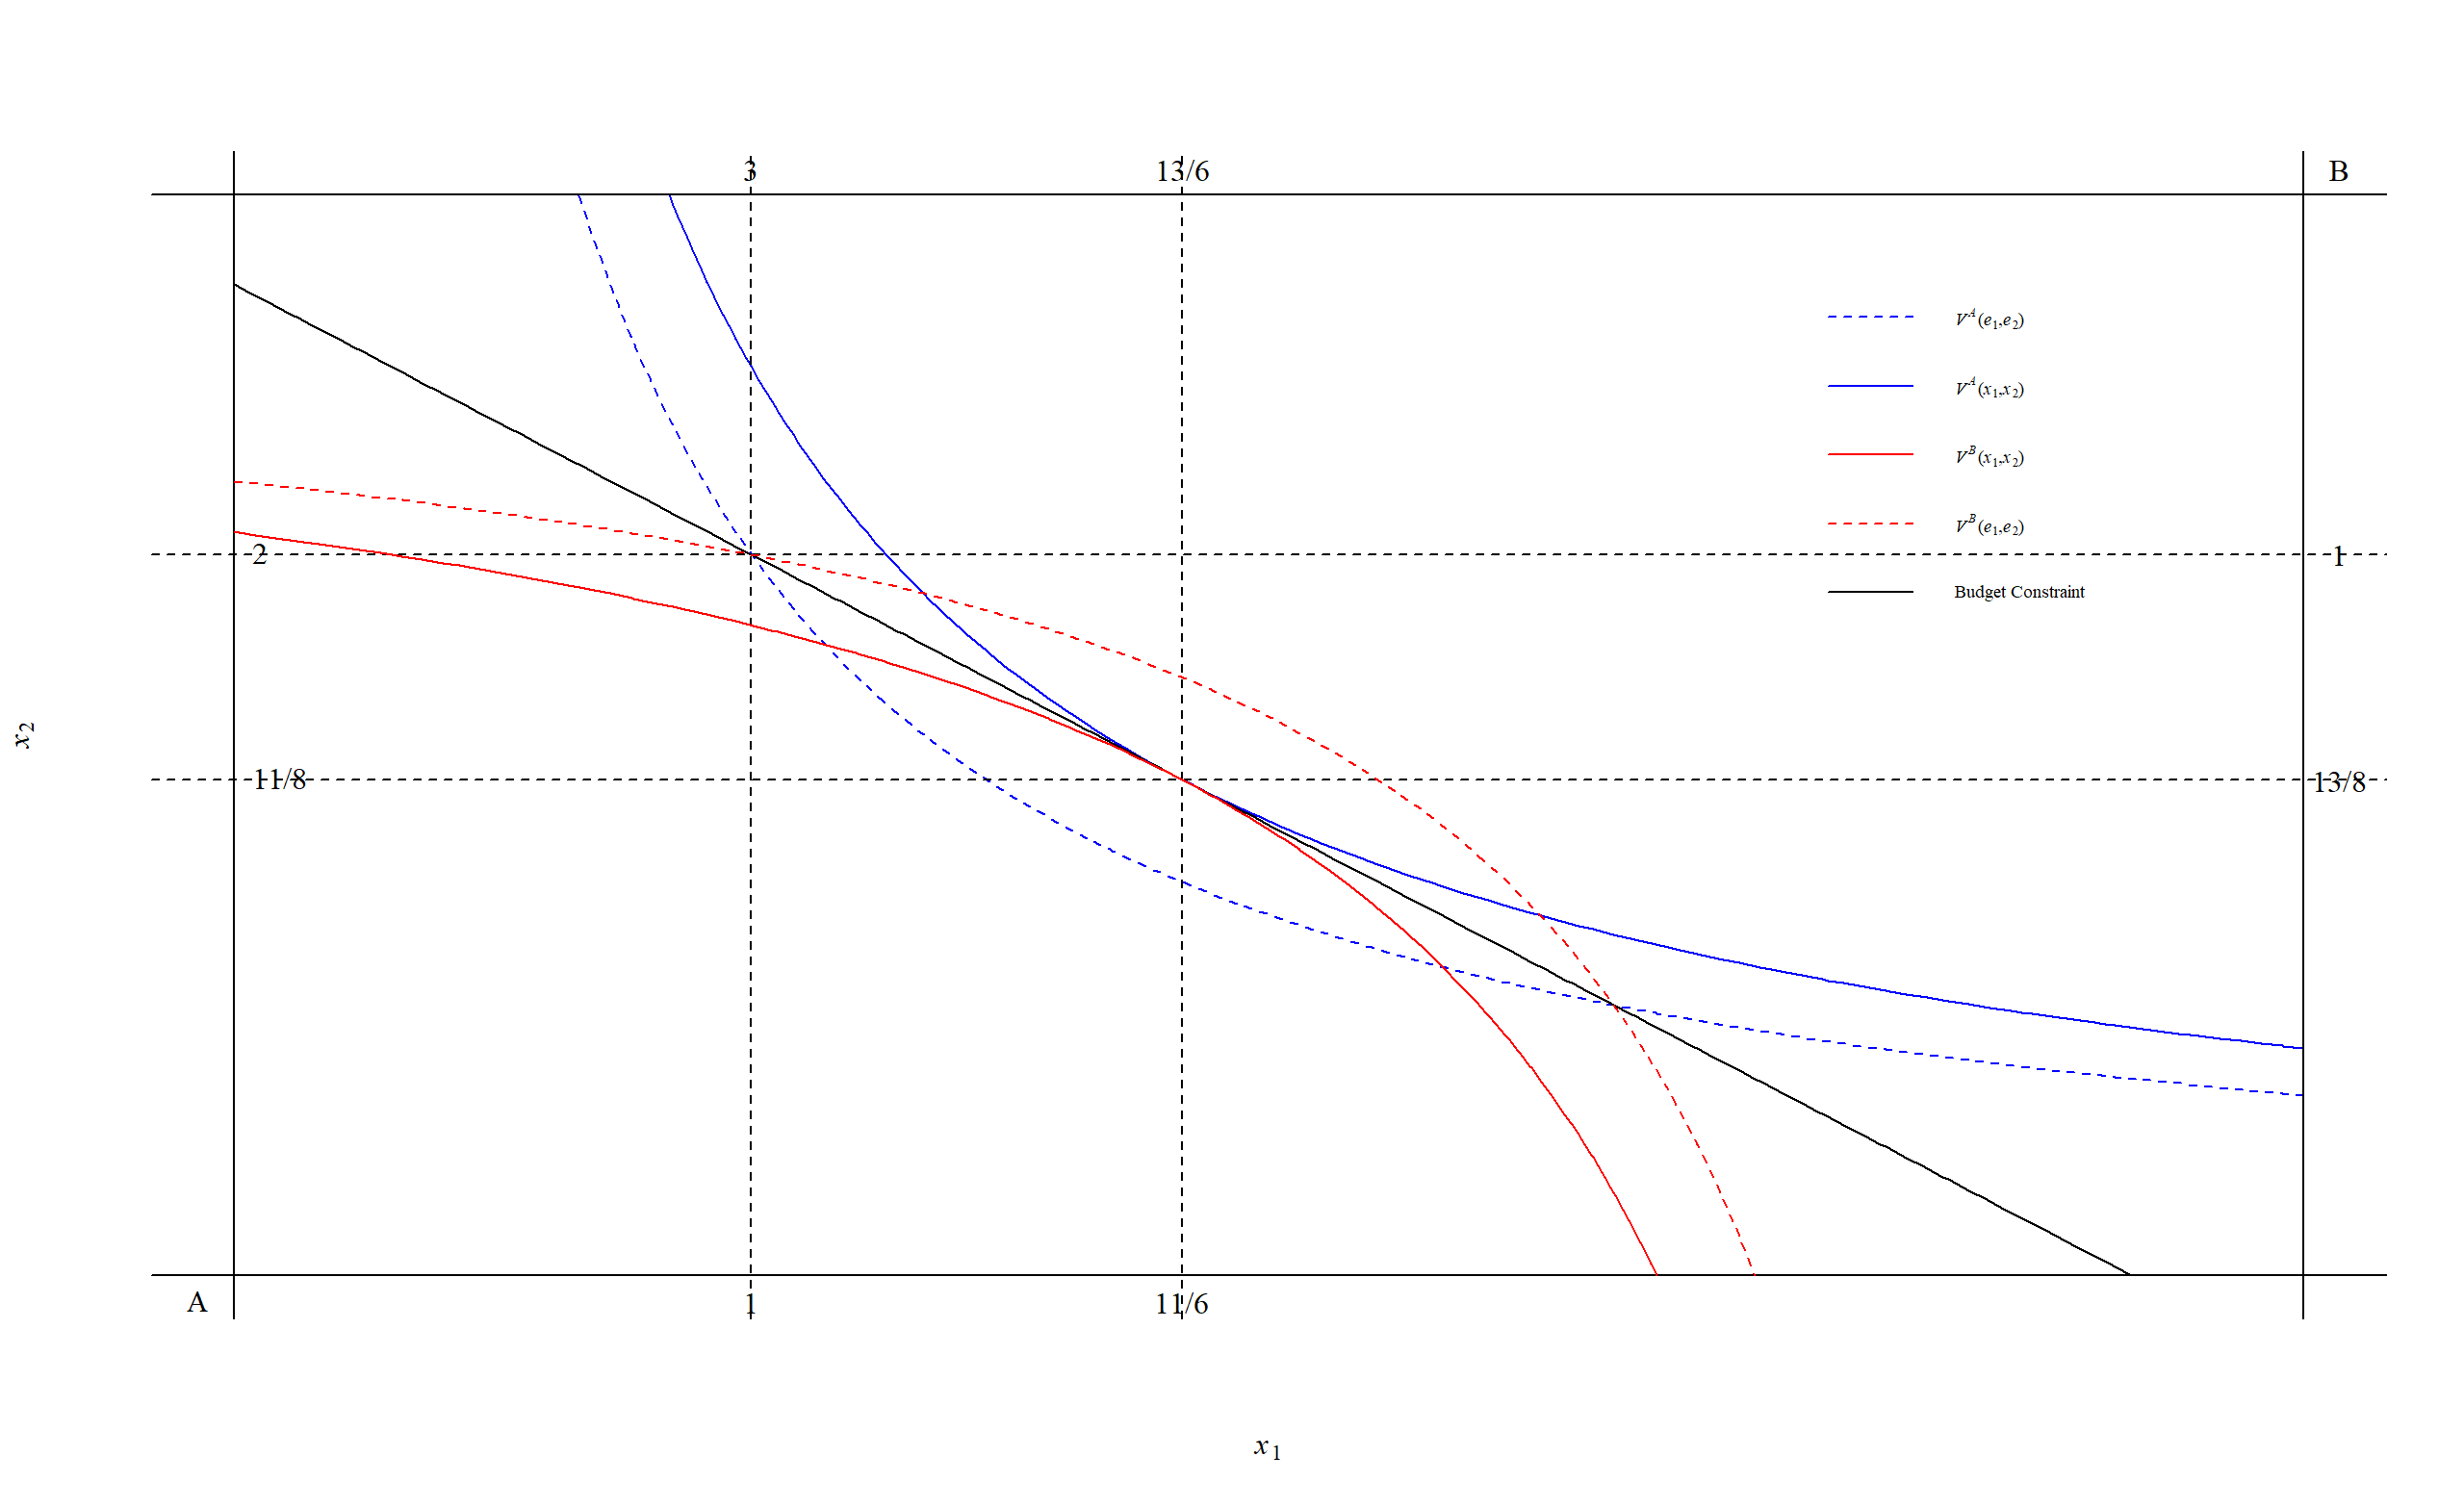
\includegraphics[width=.85\textwidth]{figures/figure3.png}
    \end{center}
    \caption{Edgeworth box diagram for Problem 3 equilibrium}
    \label{fig:graph}
\end{figure}

It's impossible to increase one's utility without hurting the other one. Thus it is Pareto optimal.

\section*{4}

\subsection*{(a)}

\fbox{%
\parbox[c]{\textwidth}{\
\begin{equation*}
    \begin{aligned}
    & \max_{\left(x^{A}_{1},x^{A}_{2}\right)}
      \dfrac{1}{3}\ln{x^{A}_{1}}+\dfrac{2}{3}\ln{x^{A}_{2}} \\
     \text{subject to}\\
    &   \hat{p}_{1}x^{A}_{1}+\hat{p}_{2}x^{A}_{2}=3\hat{p}_{1}+2\hat{p}_{2}.
    \end{aligned}
\end{equation*}%
}}

For Alice:

$MU^{A}_{1}=\dfrac{1}{3}\cdot\dfrac{1}{x^{A}_{1}}$

$MU^{A}_{2}=\dfrac{2}{3}\cdot\dfrac{1}{x^{A}_{2}}$

MRS$^{A}=\dfrac{MU^{A}_{1}}{MU^{A}_{2}}=MU^{A}_{1}\cdot\dfrac{1}{MU^{A}_{2}}=\dfrac{1}{3}\cdot\dfrac{1}{x^{A}_{1}}\cdot\dfrac{3}{2}x^{A}_{2}=\dfrac{x^{A}_{2}}{2x^{A}_{1}}$

On the other hand, 

MRS$^{A}=\dfrac{\hat{p}_{1}}{\hat{p}_{2}}$

$\therefore \dfrac{x^{A}_{2}}{2x^{A}_{1}}=\dfrac{\hat{p}_{1}}{\hat{p}_{2}}$

Substituting $x^{A}_{2}=\dfrac{2\hat{p}_{1}}{\hat{p}_{2}}x^{A}_{1}$ into budget constraint for Alice:

$\hat{p}_{1}x^{A}_{1}+\hat{p}_{2}\dfrac{2\hat{p}_{1}}{\hat{p}_{2}}x^{A}_{1}=3\hat{p}_{1}+2\hat{p}_{2}$

$\implies \hat{p}_{1}x^{A}_{1}+2\hat{p}_{1}x^{A}_{1}=3\hat{p}_{1}+2\hat{p}_{2}$

$\implies 3\hat{p}_{1}x^{A}_{1}=3\hat{p}_{1}+2\hat{p}_{2}$

$\implies x^{A}_{1}=\dfrac{3\hat{p}_{1}+2\hat{p}_{2}}{3\hat{p}_{1}}=\boxed{1+\dfrac{2}{3}\cdot\dfrac{\hat{p}_{2}}{\hat{p}_{1}}}$

$x^{A}_{2}=\dfrac{2\hat{p}_{1}}{\hat{p}_{2}}x^{A}_{1}=\dfrac{2\hat{p}_{1}}{\hat{p}_{2}}\left(1+\dfrac{2}{3}\cdot\dfrac{\hat{p}_{2}}{\hat{p}_{1}}\right)=\boxed{\dfrac{2\hat{p}_{1}}{\hat{p}_{2}}+\dfrac{4}{3}}$

\subsection*{(b)}

\fbox{%
\parbox[c]{\textwidth}{\
\begin{equation*}
    \begin{aligned}
    & \max_{\left(x^{B}_{1},x^{B}_{2}\right)}
      \dfrac{1}{2}\ln{x^{B}_{1}}+\dfrac{1}{2}\ln{x^{B}_{2}} \\
     \text{subject to}\\
    &   \hat{p}_{1}x^{B}_{1}+\hat{p}_{2}x^{B}_{2}=\hat{p}_{1}+2\hat{p}_{2}.
    \end{aligned}
\end{equation*}%
}}

For Bob:

$MU^{B}_{1}=\dfrac{1}{2}\cdot\dfrac{1}{x^{B}_{1}}$

$MU^{B}_{2}=\dfrac{1}{2}\cdot\dfrac{1}{x^{B}_{2}}$

MRS$^{B}=\dfrac{MU^{B}_{1}}{MU^{B}_{2}}=MU^{B}_{1}\cdot\dfrac{1}{MU^{B}_{2}}=\dfrac{1}{2}\cdot\dfrac{1}{x^{B}_{1}}\cdot2x^{B}_{2}=\dfrac{x^{B}_{2}}{x^{B}_{1}}$

On the other hand, 

MRS$^{B}=\dfrac{\hat{p}_{1}}{\hat{p}_{2}}$

$\therefore \dfrac{x^{B}_{2}}{x^{B}_{1}}=\dfrac{\hat{p}_{1}}{\hat{p}_{2}}$

Substituting $x^{B}_{2}=\dfrac{\hat{p}_{1}}{\hat{p}_{2}}x^{B}_{1}$ into budget constraint for Bob:

$\hat{p}_{1}x^{B}_{1}+\hat{p}_{2}\dfrac{\hat{p}_{1}}{\hat{p}_{2}}x^{B}_{1}=\hat{p}_{1}+2\hat{p}_{2}$

$\implies \hat{p}_{1}x^{B}_{1}+\hat{p}_{1}x^{B}_{1}=\hat{p}_{1}+2\hat{p}_{2}$

$\implies 2\hat{p}_{1}x^{B}_{1}=\hat{p}_{1}+2\hat{p}_{2}$

$\implies x^{B}_{1}=\dfrac{\hat{p}_{1}+2\hat{p}_{2}}{2\hat{p}_{1}}=\boxed{\dfrac{1}{2}+\dfrac{\hat{p}_{2}}{\hat{p}_{1}}}$

$x^{B}_{2}=\dfrac{\hat{p}_{1}}{\hat{p}_{2}}x^{B}_{1}=\dfrac{\hat{p}_{1}}{\hat{p}_{2}}\left(\dfrac{1}{2}+\dfrac{\hat{p}_{2}}{\hat{p}_{1}}\right)=\boxed{\dfrac{\hat{p}_{1}}{2\hat{p}_{2}}+1}$

\subsection*{(c)}

The market for consumption in state 1: 

$x^{A}_{1}+x^{B}_{1}=e^{A}_{1}+e^{B}_{1}=3+1=4$

$\iff 1+\dfrac{2}{3}\cdot\dfrac{\hat{p}_{2}}{\hat{p}_{1}}+\dfrac{1}{2}+\dfrac{\hat{p}_{2}}{\hat{p}_{1}}=4$

$\iff \left(\dfrac{2}{3}+1\right)\cdot\dfrac{\hat{p}_{2}}{\hat{p}_{1}}+\dfrac{1}{2}=3$

$\iff \dfrac{5}{3}\cdot\dfrac{\hat{p}_{2}}{\hat{p}_{1}}=\dfrac{5}{2}$

$\iff \dfrac{\hat{p}_{2}}{\hat{p}_{1}}=\dfrac{5}{2}\times\dfrac{3}{5}$

$\iff \boxed{\dfrac{\hat{p}_{1}}{\hat{p}_{2}}=\dfrac{2}{3}}$

$x^{A}_{1}=1+\dfrac{2}{3}\cdot\dfrac{\hat{p}_{2}}{\hat{p}_{1}}=1+\dfrac{2}{3}\cdot\dfrac{3}{2}=2$

$x^{B}_{1}=\dfrac{1}{2}+\dfrac{\hat{p}_{2}}{\hat{p}_{1}}=\dfrac{1}{2}+\dfrac{3}{2}=2$

$x^{A}_{2}=\dfrac{2\hat{p}_{1}}{\hat{p}_{2}}x^{A}_{1}=2\times\dfrac{2}{3}\times2=\dfrac{8}{3}$

$x^{B}_{2}=\dfrac{\hat{p}_{1}}{\hat{p}_{2}}x^{B}_{1}=\dfrac{2}{3}\times2=\dfrac{4}{3}$

Alice and Bob bear some risk: 

$x^{A}_{1}\neq x^{A}_{2}$, $x^{B}_{1}\neq x^{B}_{2}$

They hedge some risks, but not completely, to maximize their expected utility.

\subsection*{(d)}

\begin{figure}[H]
    \begin{center}
        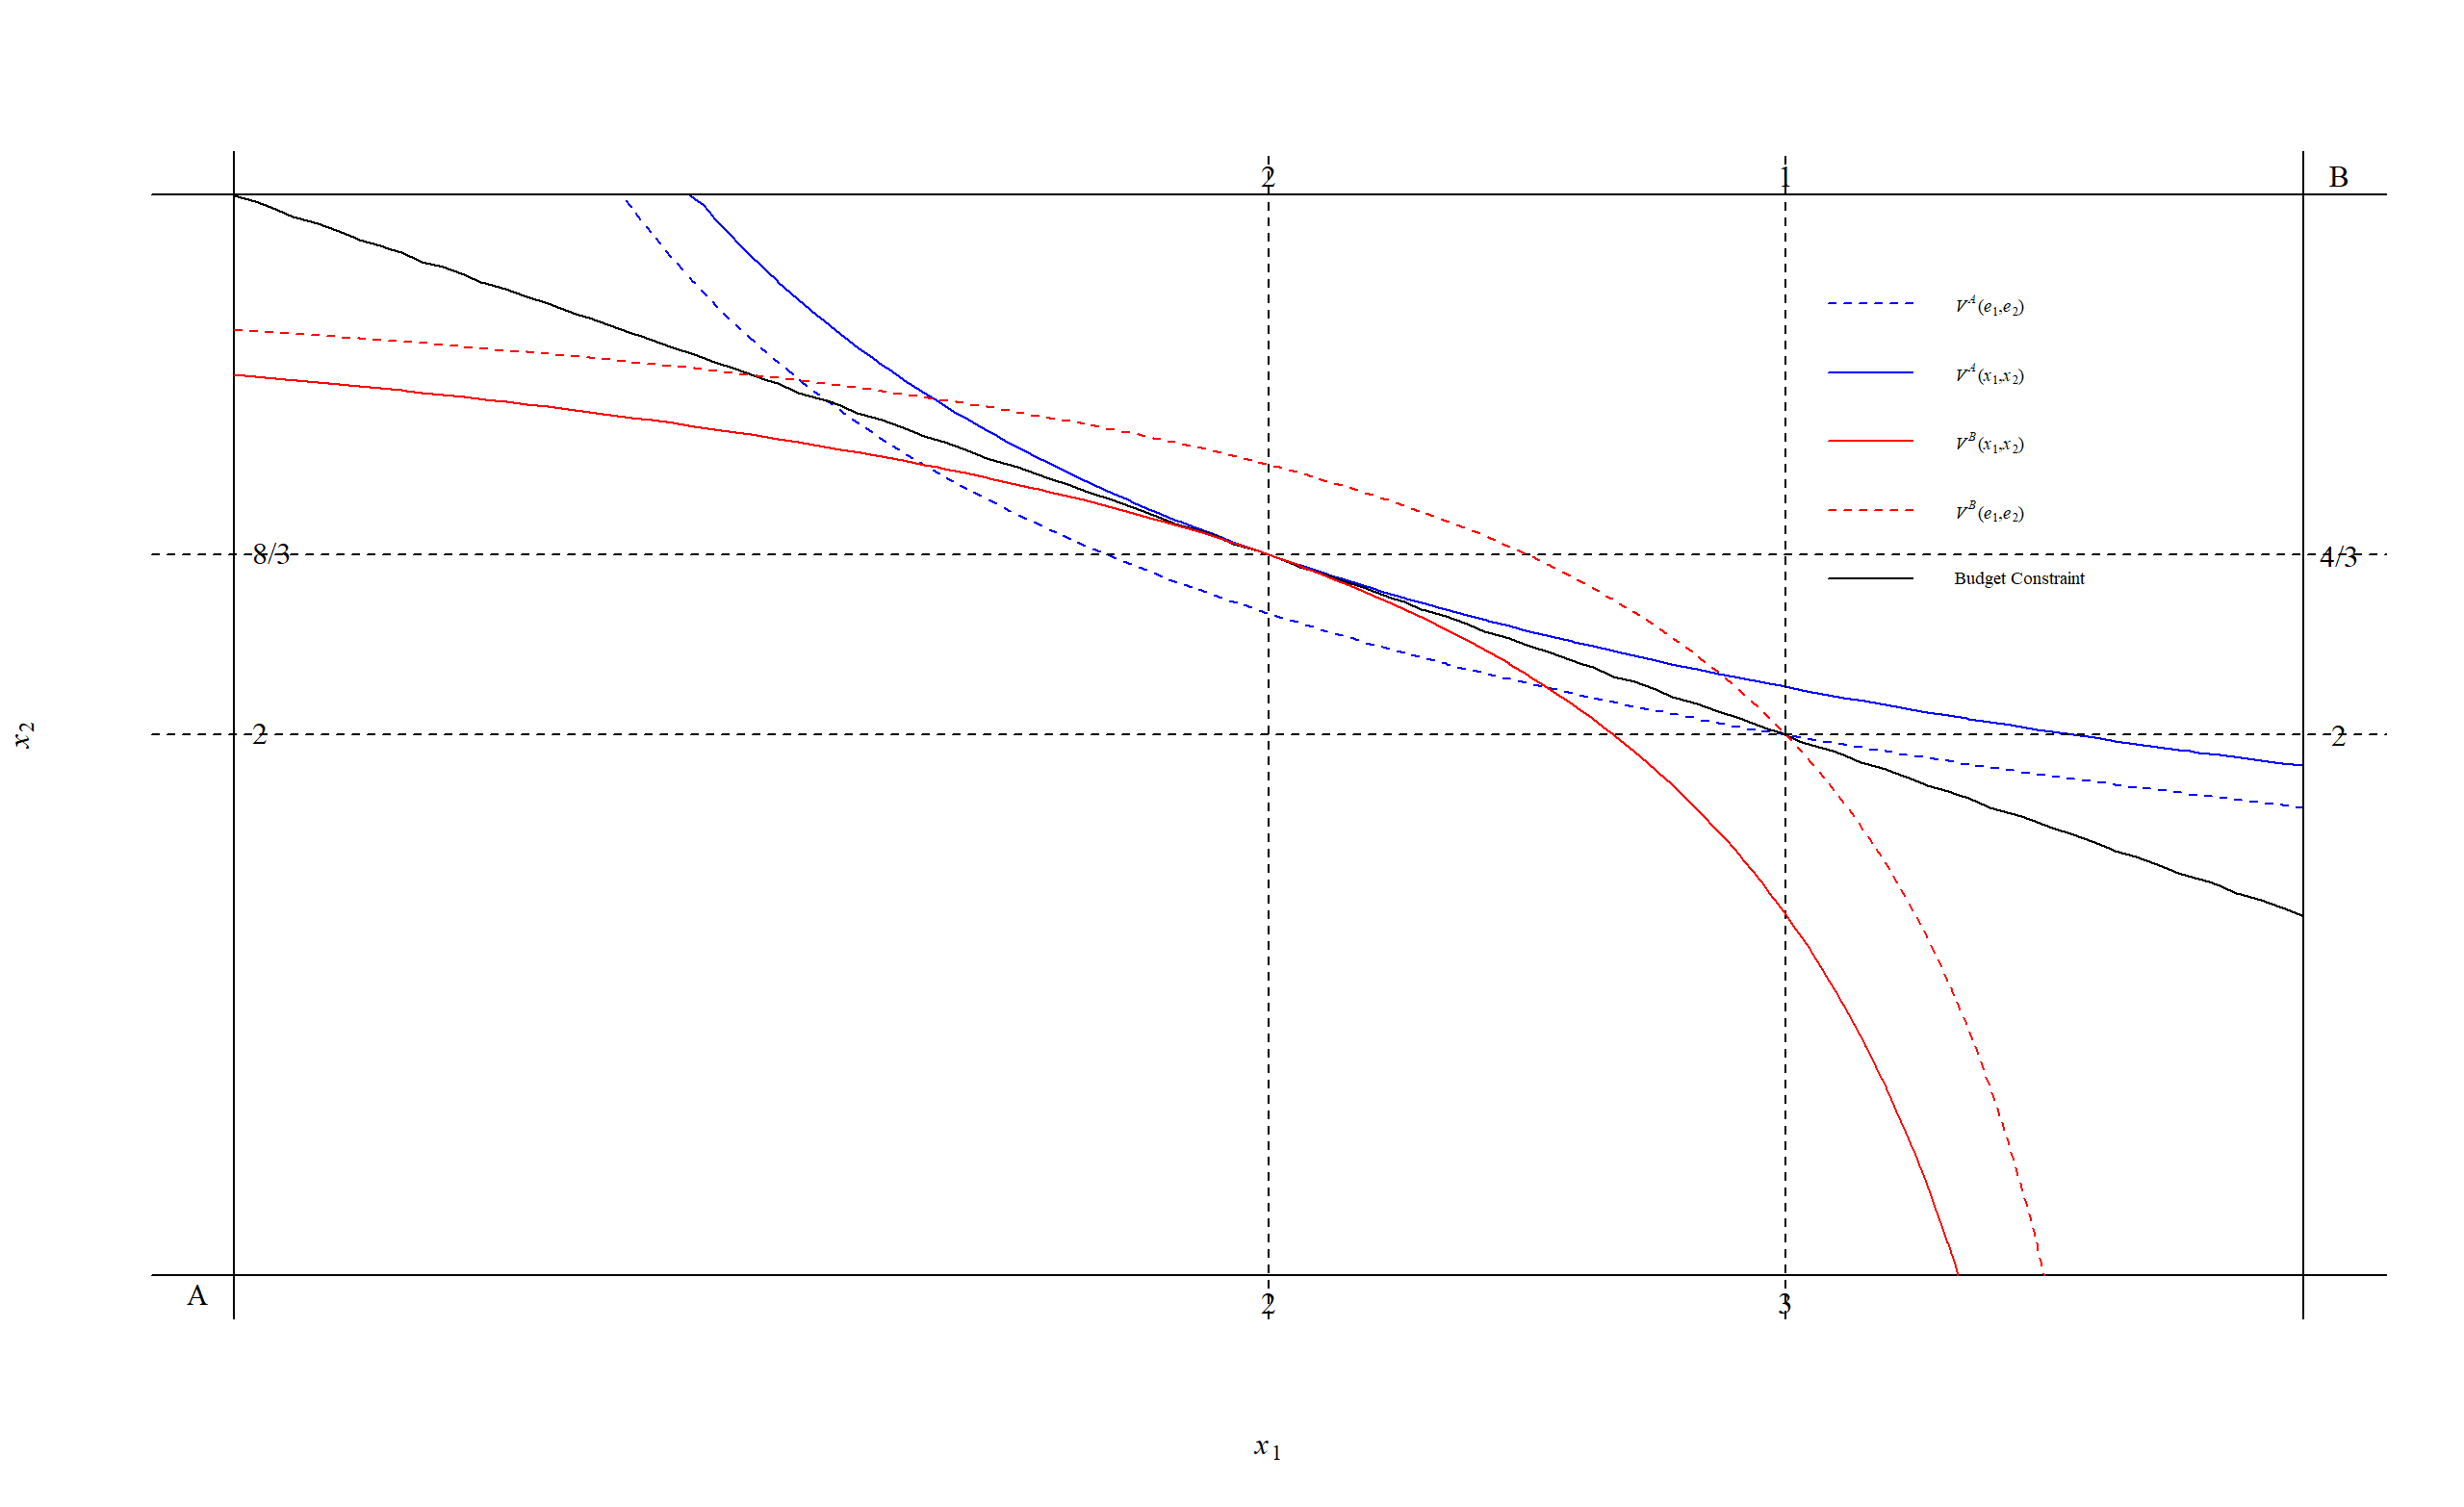
\includegraphics[width=.85\textwidth]{figures/figure4.png}
    \end{center}
    \caption{Edgeworth box diagram for Problem 4 equilibrium}
    \label{fig:graph}
\end{figure}

It's impossible to increase one's utility without hurting the other one. Thus it is Pareto optimal.

\end{document}